% gcodepreview.tex
% Author: William F. Adams (willadams at aol dot com)
% Copyright 2021--24 William F. Adams
%
% This work may be distributed and/or modified under the
% conditions of the GNU LESSER GENERAL PUBLIC LICENSE
% Version 2.1, February 1999
%
% This work consists of the files listed in the README file.
%
% 
% 
\documentclass{ltxdoc}
%https://tex.stackexchange.com/questions/722886/how-to-write-out-multiple-text-files-from-multiple-instances-of-latex-environmen
\usepackage{literati}
\usepackage[paper=legalpaper,left=1.75in,right=0.75in,top=1in,bottom=1in]{geometry}

\begin{document}

%\DoNotIndex{\bullet}

%\changes{v0.5}{2024/08/10}{DXFs and images}
\def\fileversion{v0.5} \def\filedate{2024/08/10}

%\changes{v0.4}{2024/07/28}{Literary re-write}
%\def\fileversion{v0.4} \def\filedate{2024/07/28}

%\changes{v0.3}{2024/07/01}{Curves and roundover tooling}
%\def\fileversion{v0.3} \def\filedate{2024/07/01}

%\changes{v0.2}{2024/04/12}{Initial conversion to DTX}
%\def\dtxfile{gcodepreview.dtx}

\title{The gcodepreview OpenSCAD library\thanks{This
        file (\texttt{\jobname}) has version number \fileversion, last revised
        \filedate.}}

\author{%
Author: William F. Adams\\
\texttt{willadams at aol dot com}
}
\date{\filedate}
\maketitle
\begin{abstract}
\noindent The gcodepreview library allows using OpenPythonSCAD to move a tool in lines 
and arcs and output dxf and G-code files so as to work as a CAD/\allowbreak CAM program 
for CNC.
\end{abstract}
%\enlargethispage{\baselineskip}
\tableofcontents

\clearpage
\section{readme.md}

\begin{readme}
# gcodepreview

OpenSCAD library for moving a tool in lines and arcs 
so as to model how a part would be cut using G-Code, 
so as to allow OpenSCAD to function as a compleat 
CAD/CAM solution for subtractive 3-axis CNC (mills  
and routers) by writing out G-code (in some cases 
toolpaths which would not normally be feasible), 
and to write out DXF files which may be imported 
into a traditional CAM program to create toolpaths.

![OpenSCAD Cut Joinery Module](https://raw.githubusercontent.com/WillAdams/gcodepreview/main/openscad_cutjoinery.png?raw=true)

Updated to make use of Python in OpenSCAD:[^rapcad]

[^rapcad]: Previous versions had used RapCAD, so as to take advantage of the writeln command, which has since been re-written in Python.

https://pythonscad.org/ (previously this was http://www.guenther-sohler.net/openscad/ )

A BlockSCAD file for the initial version of the 
main modules is available at:

https://www.blockscad3d.com/community/projects/1244473

The project is discussed at:

https://forum.makerforums.info/t/g-code-preview-using-openscad-rapcad/85729 

and

https://forum.makerforums.info/t/openscad-and-python-looking-to-finally-be-resolved/88171

and

https://willadams.gitbook.io/design-into-3d/programming

Since it is now programmed using Literate Programming 
(initially a .dtx, now a .tex file) there is a PDF:
https://github.com/WillAdams/gcodepreview/blob/main/gcodepreview.pdf
which includes all of the source code with formatted 
commentary.

The files for this library are:

 - gcodepreview.py (gcpy) --- the Python functions and variables
 - pygcodepreview.scad (pyscad) --- the Python functions wrapped in OpenSCAD
 - gcodepreview.scad (gcpscad) --- OpenSCAD modules and variables
 - gcodepreview_template.scad (gcptmpl) --- example file
 - cut2Dshapes.scad (cut2D) --- code for cutting 2D shapes 

Place the files in C:\Users\\\~\Documents\OpenSCAD\libraries and call as:[^libraries]

[^libraries]: C:\Users\\\~\Documents\RapCAD\libraries is deprecated since RapCAD is no longer needed since Python is now used for writing out files)

    use <gcodepreview.py>;
    use <pygcodepreview.scad>;
    include <gcodepreview.scad>;

Note that it is necessary to use the first two files 
(this allows loading the Python commands and then 
wrapping them in OpenSCAD commands) and then include 
the last file (which allows using OpenSCAD variables 
to selectively implement the Python commands via their 
being wrapped in OpenSCAD modules) and define 
variables which match the project and then use 
commands such as:

    opengcodefile(Gcode_filename);
    opendxffile(DXF_filename);
    
    difference() {
        setupstock(stocklength, stockwidth, stockthickness, zeroheight, stockorigin);
    
    movetosafez();
    
    toolchange(squaretoolno,speed * square_ratio);
    
    begintoolpath(0,0,0.25);
    beginpolyline(0,0,0.25);

    cutoneaxis_setfeed("Z",-1,plunge*square_ratio);
    addpolyline(stocklength/2,stockwidth/2,-stockthickness);
    
    cutwithfeed(stocklength/2,stockwidth/2,-stockthickness,feed);
    
    endtoolpath();
    endpolyline();
    
    }
    
    closegcodefile();
    closedxffile();

which makes a G-code file:

![OpenSCAD template G-code file](https://raw.githubusercontent.com/WillAdams/gcodepreview/main/gcodepreview_template.png?raw=true)

but one which could only be sent to a machine so as to 
cut only the softest and most yielding of materials 
since it makes a single full-depth pass, and of which 
has a matching DXF which may be imported into a 
CAM tool --- but which it is not directly possible 
to assign a toolpath in readily available CAM tools 
(since it varies in depth from beginning-to-end). 

Importing this DXF and actually cutting it 
is discussed at:

https://forum.makerforums.info/t/rewriting-gcodepreview-with-python/88617/14

Tool numbers match those of tooling sold by Carbide 3D 
(ob. discl., I work for them). 

Comments are included in the G-code to match those 
expected by CutViewer.

A complete example file is: gcodepreview_template.scad 
and another example is openscad_gcodepreview_cutjoinery.tres.scad 
which is made from an OpenSCAD Graph Editor file:

![OpenSCAD Graph Editor Cut Joinery File](https://raw.githubusercontent.com/WillAdams/gcodepreview/main/OSGE_cutjoinery.png?raw=true)

Version 0.1 supports setting up stock, origin, rapid 
positioning, making cuts, and writing out matching 
G-code, and creating a DXF with polylines.

Added features since initial upload:

 - endpolyline(); --- this command allows ending one polyline so as to allow multiple lines in a DXF
 - separate dxf files are written out for each tool where tool is ball/square/V and small/large (10/31/23)
 - re-writing as a Literate Program using the LaTeX package docmfp (begun 4/12/24) 
 - support for additional tooling shapes such as dovetail and keyhole tools

Version 0.2 adds support for arcs 

 - DXF: support for arcs (which may be used to make circles) (6/1/24)
 - Specialty toolpaths such as Keyhole which may be used for dovetail as well as keyhole cutters

Version 0.3 

 - Support for curves along the 3rd dimension
 - support for roundover tooling
 
Version 0.4

 - Rewrite using literati documentclass, suppression of SVG code
 - dxfrectangle (without G-code support)

Version 0.5

 - more shapes
 - consolidate rectangles, arcs, and circles in gcodepreview.scad

Possible future improvements:

 - support for additional tooling shapes such as tapered ball-nose tools or lollipop cutters or thread-cutting tools
 - G-code: support for G2/G3 arcs and circles
 - G-code: import external tool libraries and feeds and speeds from JSON or CSV files ---
 - general coding improvements --- current coding style is quite prosaic
 - additional generalized modules for cutting out various shapes/geometries

Note for G-code generation that it is up to the user 
to implement Depth per Pass so as to not take a 
single full-depth pass. Working from a DXF of course 
allows one to off-load such considerations to a 
specialized CAM tool.

Deprecated feature:

 - exporting SVGs --- while this was begun, it turns out that these would be written out upside down due to coordinate system differences between OpenSCAD/DXFs and SVGs requiring managing the inversion of the coordinate system (it is possible that METAPOST, which shares the same orientation and which can write out SVGs will be used instead for future versions)

\end{readme}

\clearpage
\section{gcodepreview}

This library for OpenPythonSCAD works by using Python code as a back-end so as to persistently store 
and access variables, and to write out files while both modeling the motion of a 3-axis CNC machine
and if desired, writing out DXF and/or G-code files (as opposed to the normal technique of 
rendering to a 3D model and writing out an STL). Doing so requires a total of three files:

\begin{itemize}
\item A Python file: gcodepreview.py (\texttt{gcpy}) --- this will have variables in the 
      traditional sense which may be used for tracking machine position and so forth
\item An OpenSCAD file: pygcodepreview.scad (\texttt{pyscad}) --- which wraps the Python code 
      in OpenSCAD
\item An OpenSCAD file: gcodepreview.scad (\texttt{gcpscad}) --- which uses the other two files 
      and which is \texttt{include}d allowing it to access OpenSCAD variables for branching   
\end{itemize}
 
Each file will begin with a suitable comment indicating the file type and suitable notes:

\begin{writecode}{w}{gcodepreview.py}{python}
#!/usr/bin/env python
#icon "C:\Program Files\OpenSCAD\bin\openscad.exe" --trust-python
#Currently tested with 2023.11.30 and Python 3.11
#gcodepreview 0.5, see gcodepreview.scad

\end{writecode}
\addtocounter{gcpy}{6}

\begin{writecode}{w}{pygcodepreview.scad}{scad}
//!OpenSCAD
 
//gcodepreview 0.5, see gcodepreview.scad

\end{writecode}
\addtocounter{pyscad}{5}

\begin{writecode}{w}{gcodepreview.scad}{scad}
//!OpenSCAD
 
//gcodepreview 0.5
//
//used via use <gcodepreview.py>;
//         use <pygcodepreview.scad>;
//         include <gcodepreview.scad>;
//

\end{writecode}
\addtocounter{gcpscad}{10}

The original implementation in RapSCAD used a command \DescribeRoutine{writeln} --- fortunately, 
this command is easily re-created in Python:

\lstset{firstnumber=\thegcpy}
\begin{writecode}{a}{gcodepreview.py}{python}
def writeln(*arguments):
    line_to_write = ""
    for element in arguments:
        line_to_write += element
    f.write(line_to_write)
    f.write("\n")
    
\end{writecode}
\addtocounter{gcpy}{7}

\noindent which command will accept a series of arguments and then write them out to a file 
object.

\subsection{Position and Variables}
 
In modeling the machine motion and G-code it will be necessary to have the machine track 
several variables for machine position, current tool, depth in toolpath, \&c. 
This will be done using paired functions (which will set and return the  
matching variable) and a matching (global) variable, as well as additional functions for 
setting the matching variable(s).

\begin{samepage}
The first such variables are for XYZ position:

\begin{itemize}
 \item \DescribeVariable{mpx}
 \item \DescribeVariable{mpy}
 \item \DescribeVariable{mpz}
\end{itemize}
\end{samepage}

\begin{samepage}
\noindent Similarly, for some toolpaths it will be necessary to track the depth along the Z-axis
as the toolpath is cut out:
 
\begin{itemize}
 \item \DescribeVariable{tpz}
\end{itemize}
\end{samepage}

\begin{samepage}
\noindent It will further be necessary to have a variable for the current tool:

\begin{itemize}
 \item \DescribeVariable{currenttool}
\end{itemize}
\end{samepage}

For each intended command it will be necessary to implement an appropriate aspect in each file. 
The Python file will manage the Python variables and handle things which can only be done in 
Python, while there will be two OpenSCAD files as noted above, one which calls the Python code 
(this will be \texttt{use}d), while the other will be able to access
and use OpenSCAD variables, as well as implement Customizer options
(this will be \texttt{include}d).

Note that as a convention, where it is necessary for a module to coordinate between 
Python~and OpenSCAD, it will be necessary for there to be three separate versions:
a \texttt{p}<foo>~Python definition for the manipulation of Python variables and
any file routines, an \texttt{o}<foo> OpenSCAD module which will wrap up the Python
function call, and lastly a <foo> OpenSCAD module which will be \texttt{<include>}d 
so as to be able to make use of OpenSCAD variables.

The first such routine, (actually a subroutine, see \DescribeRoutine{setupstock}) 
\DescribeSubroutine{setupstock}{psetupstock} will be appropriately enough, 
to set up the stock, and perform other initializations --- in Python all that needs 
to be done is to set the value of the persistent (Python) variables:

\lstset{firstnumber=\thegcpy}
\begin{writecode}{a}{gcodepreview.py}{python}
def psetupstock(stocklength, stockwidth, stockthickness, zeroheight, stockorigin):
    global mpx
    mpx = float(0)
    global mpy
    mpy = float(0)
    global mpz
    mpz = float(0)
    global tpz
    tpz = float(0)
    global currenttool
    currenttool = 102

\end{writecode}
\addtocounter{gcpy}{12}

The intermediary OpenSCAD code, \DescribeSubroutine{setupstock}{osetupstock} simply 
calls the Python version. Note that while the parameters are passed all the way down 
(for consistency) they are not used.

\lstset{firstnumber=\thepyscad}
\begin{writecode}{a}{pygcodepreview.scad}{scad}
 module osetupstock(stocklength, stockwidth, stockthickness, zeroheight, stockorigin) {
     psetupstock(stocklength, stockwidth, stockthickness, zeroheight, stockorigin);
 }
 
\end{writecode}
\addtocounter{pyscad}{4}

The OpenSCAD code, \DescribeRoutine{setupstock} requires that the user set parameters
for stock dimensions and so forth, and will create comments in the G-code which incorporate 
the stock dimensions and its position relative to the zero as set relative to the stock.
 
The \DescribeVariable{stockorigin} setting is used in an <if then else> structure to position
the 3D model of the stock. 

\lstset{firstnumber=\thepyscad}
\begin{writecode}{a}{pygcodepreview.scad}{scad}
module setupstock(stocklength, stockwidth, stockthickness, zeroheight, stockorigin) {
  osetupstock(stocklength, stockwidth, stockthickness, zeroheight, stockorigin);
//initialize default tool and XYZ origin
  osettool(102);
  oset(0,0,0);
  if (zeroheight == "Top") {
    if (stockorigin == "Lower-Left") {
    translate([0, 0, (-stockthickness)]){
    cube([stocklength, stockwidth, stockthickness], center=false);
      if (generategcode == true) {
      owritethree("(stockMin:0.00mm, 0.00mm, -",str(stockthickness),"mm)");
      owritefive("(stockMax:",str(stocklength),"mm, ",str(stockwidth),"mm, 0.00mm)");
      owritenine("(STOCK/BLOCK, ",str(stocklength),", ",str(stockwidth),", ",str(stockthickness),", 0.00, 0.00, ",str(stockthickness),")");
    }
  }
}
     else if (stockorigin == "Center-Left") {
    translate([0, (-stockwidth / 2), -stockthickness]){
      cube([stocklength, stockwidth, stockthickness], center=false);
    if (generategcode == true) {
owritefive("(stockMin:0.00mm, -",str(stockwidth/2),"mm, -",str(stockthickness),"mm)");
owritefive("(stockMax:",str(stocklength),"mm, ",str(stockwidth/2),"mm, 0.00mm)");
    owriteeleven("(STOCK/BLOCK, ",str(stocklength),", ",str(stockwidth),", ",str(stockthickness),", 0.00, ",str(stockwidth/2),", ",str(stockthickness),")");
    }
  }
    } else if (stockorigin == "Top-Left") {
    translate([0, (-stockwidth), -stockthickness]){
      cube([stocklength, stockwidth, stockthickness], center=false);
if (generategcode == true) {
owritefive("(stockMin:0.00mm, -",str(stockwidth),"mm, -",str(stockthickness),"mm)");
owritethree("(stockMax:",str(stocklength),"mm, 0.00mm, 0.00mm)");
owriteeleven("(STOCK/BLOCK, ",str(stocklength),", ",str(stockwidth),", ",str(stockthickness),", 0.00, ",str(stockwidth),", ",str(stockthickness),")");
    }
  }
    }
    else if (stockorigin == "Center") {
//owritecomment("Center");
    translate([(-stocklength / 2), (-stockwidth / 2), -stockthickness]){
      cube([stocklength, stockwidth, stockthickness], center=false);
if (generategcode == true) {
owriteseven("(stockMin: -",str(stocklength/2),", -",str(stockwidth/2),"mm, -",str(stockthickness),"mm)");
owritefive("(stockMax:",str(stocklength/2),"mm, ",str(stockwidth/2),"mm, 0.00mm)");
owritethirteen("(STOCK/BLOCK, ",str(stocklength),", ",str(stockwidth),", ",str(stockthickness),", ",str(stocklength/2),", ", str(stockwidth/2),", ",str(stockthickness),")");
      }
    }
  }
} else if (zeroheight == "Bottom") {
//owritecomment("Bottom");
    if (stockorigin == "Lower-Left") {
    cube([stocklength, stockwidth, stockthickness], center=false);
if (generategcode == true) {
owriteone("(stockMin:0.00mm, 0.00mm, 0.00mm)");
owriteseven("(stockMax:",str(stocklength),"mm, ",str(stockwidth),"mm, ",str(stockthickness),"mm)");
owriteseven("(STOCK/BLOCK, ",str(stocklength),", ",str(stockwidth),", ",str(stockthickness),",0.00, 0.00, 0.00)");
    }
}    else if (stockorigin == "Center-Left") {
    translate([0, (-stockwidth / 2), 0]){
      cube([stocklength, stockwidth, stockthickness], center=false);
if (generategcode == true) {
owritethree("(stockMin:0.00mm, -",str(stockwidth/2),"mm, 0.00mm)");
owriteseven("(stockMax:",str(stocklength),"mm, ",str(stockwidth/2),"mm, ",str(stockthickness),"mm)");
owritenine("(STOCK/BLOCK, ",str(stocklength),", ",str(stockwidth),", ",str(stockthickness),",0.00, ",str(stockwidth/2),", 0.00)");
    }
  } 
    } else if (stockorigin == "Top-Left") {
    translate([0, (-stockwidth), 0]){
      cube([stocklength, stockwidth, stockthickness], center=false);
    }
if (generategcode == true) {
owritethree("(stockMin:0.00mm, -",str(stockwidth),"mm, 0.00mm)");
owritefive("(stockMax:",str(stocklength),"mm, 0.00mm, ",str(stockthickness),"mm)");
owritenine("(STOCK/BLOCK, ",str(stocklength),", ",str(stockwidth),", ",str(stockthickness),", 0.00, ", str(stockwidth),", 0.00)");
  }
}    else if (stockorigin == "Center") {
    translate([(-stocklength / 2), (-stockwidth / 2), 0]){
      cube([stocklength, stockwidth, stockthickness], center=false);
    }
if (generategcode == true) {
owritefive("(stockMin:-",str(stocklength/2),", -",str(stockwidth/2),"mm, 0.00mm)");
owriteseven("(stockMax:",str(stocklength/2),"mm, ",str(stockwidth/2),"mm, ",str(stockthickness),"mm)");
owriteeleven("(STOCK/BLOCK, ",str(stocklength),", ",str(stockwidth),", ",str(stockthickness),", ",str(stocklength/2),", ", str(stockwidth/2),", 0.00)");
    }
  }
}
if (generategcode == true) {
    owriteone("G90");
    owriteone("G21");
//    owriteone("(Move to safe Z to avoid workholding)");
//    owriteone("G53G0Z-5.000");
  }
//owritecomment("ENDSETUP");
}

\end{writecode}
\addtocounter{pyscad}{93}

It will be necessary to have Python functions (\DescribeRoutine{xpos}, \DescribeRoutine{ypos}, 
and \DescribeRoutine{zpos}) which return the current values of the machine position in 
Cartesian coordinates: 

\lstset{firstnumber=\thegcpy}
\begin{writecode}{a}{gcodepreview.py}{python}
def xpos():
    global mpx
    return mpx

def ypos():
    global mpy
    return mpy

def zpos():
    global mpz
    return mpz

def tzpos():
    global tpz
    return tpz

\end{writecode}
\addtocounter{gcpy}{16}

\noindent and in turn, functions which set the positions: 
\DescribeSubroutine{setxpos}{psetxpos},
\DescribeSubroutine{setypos}{psetypos},
\DescribeSubroutine{setzpos}{psetzpos}, and
\DescribeSubroutine{settzpos}{psettzpos}

\lstset{firstnumber=\thegcpy}
\begin{writecode}{a}{gcodepreview.py}{python}
def psetxpos(newxpos):
    global mpx
    mpx = newxpos

def psetypos(newypos):
    global mpy
    mpy = newypos

def psetzpos(newzpos):
    global mpz
    mpz = newzpos
 
def psettzpos(newtzpos):
    global tpz
    tpz = newtzpos

\end{writecode}
\addtocounter{gcpy}{16}
 
\noindent and as noted above, there will need to be matching OpenSCAD versions which will 
set: \DescribeRoutine{setxpos}, \DescribeRoutine{setypos}, \DescribeRoutine{setzpos}, and
\DescribeRoutine{settzpos}; as well as return the value: \DescribeRoutine{getxpos}, \DescribeRoutine{getypos}, \DescribeRoutine{getzpos}, and \DescribeRoutine{gettzpos} 
Note that for routines where the variable is directly passed from OpenSCAD to Python
it is possible to have OpenSCAD directly call the matching Python module with no need
to use an intermediary OpenSCAD module.
 
\lstset{firstnumber=\thepyscad}
\begin{writecode}{a}{pygcodepreview.scad}{scad}
function getxpos() = xpos();
function getypos() = ypos();
function getzpos() = zpos();
function gettzpos() = tzpos();

module setxpos(newxpos) {
    psetxpos(newxpos);
}

module setypos(newypos) {
    psetypos(newypos);
}

module setzpos(newzpos) {
    psetzpos(newzpos);
}

module settzpos(newtzpos) {
    psettzpos(newtzpos);
}

\end{writecode}
\addtocounter{pyscad}{21}
 
\noindent\DescribeRoutine{oset} while for setting the variables, it is necessary to have
an OpenSCAD module:

\lstset{firstnumber=\thegcpscad}
\begin{writecode}{a}{gcodepreview.scad}{scad}
module oset(ex, ey, ez) {
    setxpos(ex);
    setypos(ey);
    setzpos(ez);
}

\end{writecode}
\addtocounter{gcpscad}{6}
 
\noindent and some toolpaths will require the storing and usage\DescribeRoutine{osettz}
of an intermediate value for the Z-axis position during calculation:

\lstset{firstnumber=\thegcpscad}
\begin{writecode}{a}{gcodepreview.scad}{scad}
module osettz(tz) {
    settzpos(tz);
}

\end{writecode}
\addtocounter{gcpscad}{4}

\subsection{Tools and Changes}
 
Similarly Python functions and variables will be used in: \DescribeRoutine{pcurrenttool} and
\DescribeRoutine{psettool} to track and set and return the current tool
 
\lstset{firstnumber=\thegcpy}
\begin{writecode}{a}{gcodepreview.py}{python}
def psettool(tn):
    global currenttool
    currenttool = tn

def pcurrent_tool():
    global currenttool
    return currenttool

\end{writecode}
\addtocounter{gcpy}{8}
 
\noindent and matching OpenSCAD modules:
\DescribeRoutine{osettool} and
\DescribeRoutine{currenttool}
set and return the current tool: 
  
\lstset{firstnumber=\thepyscad}
\begin{writecode}{a}{pygcodepreview.scad}{scad}
module osettool(tn){
    psettool(tn);
}

function current_tool() = pcurrent_tool();

\end{writecode}
\addtocounter{pyscad}{6}
 
\subsubsection{toolchange}
\noindent and apply the appropriate commands for a \label{subsubsec:toolchange}
\DescribeRoutine{toolchange}. Note that it is expected that this code will be updated as needed 
when new tooling is introduced as additional modules which require specific tooling are added below.

Note that the comments written out in G-code correspond to that used by the G-code previewing tool 
CutViewer (which is unfortunately, no longer readily available).

It is possible that rather than hard-coding the tool definitions, a future update will instead
read them in from an external file --- the \texttt{.csv} format used for tool libraries in 
Carbide Create seems a likely candidate and worth exploring.

Note that there are many varieties of tooling and not all will be implemented, especially in the 
early versions of this project
 
\begin{samepage}
\paragraph{Normal Tooling}

\label{para:normaltooling} Most tooling has quite standard shapes 
and are defined by their profile:

  \noindent
\includegraphics[width=\linewidth/3]{images/tool_square_201.png}%
           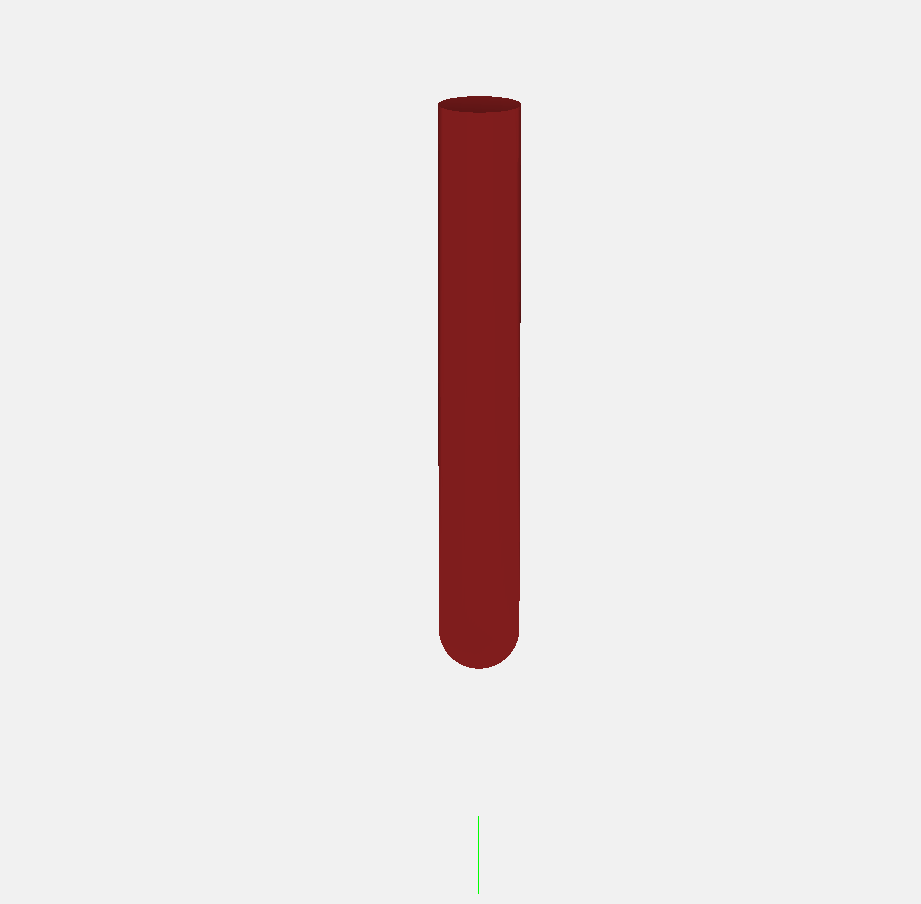
\includegraphics[width=\linewidth/3]{images/tool_ball_202.png}%
           
\includegraphics[width=\linewidth/3]{images/tool_V_301.png}%

\begin{itemize}
\item Square (\#201 and 102) --- able to cut a flat bottom, perpendicular side and right angle
                                 their simple and easily understood geometry makes them a 
                                 standard choice (a radiused form with a flat bottom, often
                                 described as a ``bowl bit'' is not implemented as-of-yet)
\item Ballnose (\#202 and 101) --- rounded, they are the standard choice for concave and 
                                   organic shapes
\item V tooling (\#301, 302 and 390) --- pointed at the tip, they are available in a variety of
                                         angles and diameters and may be used for decorative
                                         V carving, or for chamfering or cutting specific angles
                                         (note that the commonly available radiused form is not
                                         implemented at this time, \emph{e.g.},~\#501 and 502)
\end{itemize}
\end{samepage}

\lstset{firstnumber=\thegcpscad}
\begin{writecode}{a}{gcodepreview.scad}{scad}
module toolchange(tool_number,speed) {
   osettool(tool_number); 
if (generategcode == true) {
    writecomment("Toolpath");
    owriteone("M05");
//    writecomment("Move to safe Z to avoid workholding");
//    owriteone("G53G0Z-5.000");
//    writecomment("Begin toolpath");
    if (tool_number == 201) {
      writecomment("TOOL/MILL,6.35, 0.00, 0.00, 0.00");
    } else if (tool_number == 202) {
      writecomment("TOOL/MILL,6.35, 3.17, 0.00, 0.00");
    } else if (tool_number == 102) {
      writecomment("TOOL/MILL,3.17, 0.00, 0.00, 0.00");
    } else if (tool_number == 101) {
      writecomment("TOOL/MILL,3.17, 1.58, 0.00, 0.00");
    } else if (tool_number == 301) {
      writecomment("TOOL/MILL,0.03, 0.00, 6.35, 45.00");
    } else if (tool_number == 302) {
      writecommment("TOOL/MILL,0.03, 0.00, 10.998, 30.00");
    } else if (tool_number == 390) {
      writecomment("TOOL/MILL,0.03, 0.00, 1.5875, 45.00");
\end{writecode}
\addtocounter{gcpscad}{22}

\paragraph{Tooling for Keyhole Toolpaths}

\label{para:undercuttooling} Keyhole toolpaths (see: subsection~\ref{subsec:keyholetoolpaths} 
are intended for use with tooling which projects beyond the the narrower shaft and so
will cut usefully underneath the visible surface. Also described as ``undercut'' tooling,
but see below.

\begin{samepage}
There are several notable candidates for such tooling:

\begin{itemize}
\item Keyhole tools --- intended to cut slots for retaining hardware used for picture
                        hanging, they may be used to create slots for other purposes
\item Dovetail cutters --- used for the joinery of the same name, they cut a large
                           area at the bottom which slants up to a narrower region
                           at a defined angle
\item Lollipop cutters --- normally used for 3D work, as their name suggests they are
                           essentially a (cutting) ball on a narrow stick (the tool shaft),
                           they are mentioned here only for compleatness' sake and are not
                           (at this time) implemented
\end{itemize}
\end{samepage}
 
\lstset{firstnumber=\thegcpscad}
\begin{writecode}{a}{gcodepreview.scad}{scad}
   } else if (tool_number == 375) {
     writecomment("TOOL/MILL,9.53, 0.00, 3.17, 0.00");
\end{writecode}
\addtocounter{gcpscad}{2}
 
\lstset{firstnumber=\thegcpscad}
\begin{writecode}{a}{gcodepreview.scad}{scad}
   } else if (tool_number == 814) {
     writecomment("TOOL/MILL,12.7, 6.367, 12.7, 0.00");
\end{writecode}
\addtocounter{gcpscad}{2}
 
\paragraph{Thread mills}

\label{para:threadmills} The implementation of arcs cutting along the Z-axis raises the 
possibility of cutting threads using ``thread mills''. 
See: \url{https://community.carbide3d.com/t/thread-milling-in-metal-on-the-shapeoko-3/5332}

Note that it will be necessary to to define modules (see below) for each tool shape.

With the tools delineated, the module is closed out and the tooling information written into
the G-code.
 
\lstset{firstnumber=\thegcpscad}
\begin{writecode}{a}{gcodepreview.scad}{scad}
   }
     select_tool(tool_number);
     owritetwo("M6T",str(tool_number));
     owritetwo("M03S",str(speed));
 }
}

\end{writecode}
\addtocounter{gcpscad}{7}

\paragraph{Roundover tooling}

\label{para:roundover} It is not possible to represent all tools using tool changes 
as coded above which require using a \texttt{hull} operation between 3D representations
of the tools at the beginning and end points. Tooling which cannot be so represented will be implemented separately below, see paragraph~\ref{para:concavetoolshapes}.

\paragraph{Selecting Tools}

There must also be a module for selecting tools: \DescribeRoutine{selecttool} which will
select the matching module for 3D modeling based on the \DescribeVariable{tool number}, 
and pass the appropriate parameters to that module:
 
\lstset{firstnumber=\thegcpscad}
\begin{writecode}{a}{gcodepreview.scad}{scad}
module select_tool(tool_number) {
//echo(tool_number);
  if (tool_number == 201) {
    gcp_endmill_square(6.35, 19.05);
  } else if (tool_number == 202) {
    gcp_endmill_ball(6.35, 19.05);
  } else if (tool_number == 102) {
    gcp_endmill_square(3.175, 19.05);
  } else if (tool_number == 101) {
    gcp_endmill_ball(3.175, 19.05);
  } else if (tool_number == 301) {
    gcp_endmill_v(90, 12.7);
  } else if (tool_number == 302) {
    gcp_endmill_v(60, 12.7);
  } else if (tool_number == 390) {
    gcp_endmill_v(90, 3.175);
\end{writecode}
\addtocounter{gcpscad}{16}
 
For a keyhole tool:
 
\lstset{firstnumber=\thegcpscad}
\begin{writecode}{a}{gcodepreview.scad}{scad}
  } else if (tool_number == 375) {
    gcp_keyhole(9.525, 3.175);
\end{writecode}
\addtocounter{gcpscad}{2}
 
\noindent and dovetail tool:
 
\lstset{firstnumber=\thegcpscad}
\begin{writecode}{a}{gcodepreview.scad}{scad}
  } else if (tool_number == 814) {
    gcp_dovetail(12.7, 6.367, 12.7, 14);
\end{writecode}
\addtocounter{gcpscad}{2}

Once all tools have been defined the \texttt{if} statement and module may be closed:
 
\lstset{firstnumber=\thegcpscad}
\begin{writecode}{a}{gcodepreview.scad}{scad}
  }
}

\end{writecode}
\addtocounter{gcpscad}{3}

\subsubsection{3D Shapes for Tools}

Each tool must be modeled in 3D using an OpenSCAD module. 

\paragraph{Normal toolshapes}
Most tools are easily implemented with concise 3D descriptions which may be connected with
a simple \texttt{hull} operation:

The \DescribeRoutine{gcp endmill square} is a simple cylinder:
\lstset{firstnumber=\thegcpscad}
\begin{writecode}{a}{gcodepreview.scad}{scad}
module gcp_endmill_square(es_diameter, es_flute_length) {
  cylinder(r1=(es_diameter / 2), r2=(es_diameter / 2), h=es_flute_length, center=false);
}

\end{writecode}
\addtocounter{gcpscad}{4}

\begin{samepage}
The \DescribeRoutine{gcp keyhole} is modeled only by the the cutting base:
\lstset{firstnumber=\thegcpscad}
\begin{writecode}{a}{gcodepreview.scad}{scad}
module gcp_keyhole(es_diameter, es_flute_length) {
  cylinder(r1=(es_diameter / 2), r2=(es_diameter / 2), h=es_flute_length, center=false);
}

\end{writecode}
\addtocounter{gcpscad}{4}
\end{samepage}

The \DescribeRoutine{gcp dovetail} is modeled as a cylinder with the differing bottom and 
top diameters determining the angle (though \DescribeVariable{dt angle} is still required 
as a parameter)
\lstset{firstnumber=\thegcpscad}
\begin{writecode}{a}{gcodepreview.scad}{scad}
module gcp_dovetail(dt_bottomdiameter, dt_topdiameter, dt_height, dt_angle) {
  cylinder(r1=(dt_bottomdiameter / 2), r2=(dt_topdiameter / 2), h= dt_height, center=false);
}

\end{writecode}
\addtocounter{gcpscad}{4}

The \DescribeRoutine{gcp endmill ball} is modeled as a hemisphere joined with a cylinder:
\lstset{firstnumber=\thegcpscad}
\begin{writecode}{a}{gcodepreview.scad}{scad}
module gcp_endmill_ball(es_diameter, es_flute_length) {
  translate([0, 0, (es_diameter / 2)]){
    union(){
      sphere(r=(es_diameter / 2));
      cylinder(r1=(es_diameter / 2), r2=(es_diameter / 2), h=es_flute_length, center=false);
    }
  }
}

\end{writecode}
\addtocounter{gcpscad}{9}

The \DescribeRoutine{gcp endmill v} is modeled as a cylinder with a zero width base and
a second cylinder for the shaft:
\lstset{firstnumber=\thegcpscad}
\begin{writecode}{a}{gcodepreview.scad}{scad}
module gcp_endmill_v(es_v_angle, es_diameter) {
  union(){
    cylinder(r1=0, r2=(es_diameter / 2), h=((es_diameter / 2) / tan((es_v_angle / 2))), center=false);
    translate([0, 0, ((es_diameter / 2) / tan((es_v_angle / 2)))]){
      cylinder(r1=(es_diameter / 2), r2=(es_diameter / 2), h=((es_diameter * 8) ), center=false);/// tan((es_v_angle / 2))
    }
  }
}

\end{writecode}
\addtocounter{gcpscad}{9}
 
\paragraph{Concave toolshapes}
\label{para:concavetoolshapes} 
While normal tooling may be represented with a single \texttt{hull} operation betwixt two
3D toolshapes, concave tooling such as roundover/radius tooling require multiple slices
of the tool shape which are then \texttt{hull}ed together. Something of this can be seen
in the manual work-around for previewing them: 
\url{https://community.carbide3d.com/t/using-unsupported-tooling-in-carbide-create-roundover-cove-radius-bits/43723}.

Ideally, it would be possible to simply identify such tooling using the tool \# in the
code used for normal toolshapes as above, but the most expedient option is to simply
use a specific command for this. Since such tooling is quite limited in its use and 
normally only used at the surface of the part along an edge, this separation is 
easily justified.

Because it is necessary to divide the tooling into vertical slices and call the hull operation 
for each slice the tool definitions are tightly coupled with the module. Note that there are 
two different modules, the public-facing version which includes the tool number:
\DescribeRoutine{radiuscut}
 
\lstset{firstnumber=\thegcpscad}
\begin{writecode}{a}{gcodepreview.scad}{scad}
module radiuscut(bx, by, bz, ex, ey, ez, radiustn) {
    if (radiustn == 56125) {
        radiuscuttool(bx, by, bz, ex, ey, ez, 0.508/2, 1.531);
    } else if (radiustn == 56142) {
        radiuscuttool(bx, by, bz, ex, ey, ez, 0.508/2, 2.921);
    } else if (radiustn == 312) {
        radiuscuttool(bx, by, bz, ex, ey, ez, 1.524/2, 3.175);
    } else if (radiustn == 1570) {
        radiuscuttool(bx, by, bz, ex, ey, ez, 0.507/2, 4.509);
    }
}

\end{writecode}
\addtocounter{gcpscad}{12}

\noindent which then calls the actual \texttt{radiuscuttool} module  
passing in the tip radius and the radius of the rounding. Note that this
module sets its quality relative to the value of \verb|$fn|.

\lstset{firstnumber=\thegcpscad}
\begin{writecode}{a}{gcodepreview.scad}{scad}
module radiuscuttool(bx, by, bz, ex, ey, ez, tool_radius_tip, tool_radius_width) {
n = 90 + $fn*3;
step = 360/n;

hull(){
    translate([bx,by,bz])
    cylinder(step,tool_radius_tip,tool_radius_tip);
    translate([ex,ey,ez])
    cylinder(step,tool_radius_tip,tool_radius_tip);
}

hull(){
translate([bx,by,bz+tool_radius_width])
cylinder(tool_radius_width*2,tool_radius_tip+tool_radius_width,tool_radius_tip+tool_radius_width);

translate([ex,ey,ez+tool_radius_width])
  cylinder(tool_radius_width*2,tool_radius_tip+tool_radius_width,tool_radius_tip+tool_radius_width);
}

for (i=[0:step:90]) {
    angle = i;
    dx = tool_radius_width*cos(angle);
    dxx = tool_radius_width*cos(angle+step);
    dzz = tool_radius_width*sin(angle);
    dz = tool_radius_width*sin(angle+step);
    dh = dz-dzz;
    hull(){
        translate([bx,by,bz+dz])
            cylinder(dh,tool_radius_tip+tool_radius_width-dx,tool_radius_tip+tool_radius_width-dxx);
        translate([ex,ey,ez+dz])
            cylinder(dh,tool_radius_tip+tool_radius_width-dx,tool_radius_tip+tool_radius_width-dxx);
        }
    }
}

\end{writecode}
\addtocounter{gcpscad}{35}

\subsubsection{tooldiameter}

It will also be necessary to be able to provide the diameter of the current tool.
Arguably, this would be much easier using an object-oriented programming style/dot notation.

One aspect of tool parameters which will need to be supported is shapes which create
different profiles based on how deeply the tool is cutting into the surface of the 
material at a given point. To accommodate this, it will be necessary to either track
the thickness of uncut material at any given point, or, to specify the depth of cut 
as a parameter which is what the initial version will implement.

The public-facing OpenSCAD code, \DescribeRoutine{tool diameter}
simply calls the matching OpenSCAD module which wraps the Python code:
 
\lstset{firstnumber=\thegcpscad}
\begin{writecode}{a}{gcodepreview.scad}{scad}
function tool_diameter(td_tool, td_depth) = otool_diameter(td_tool, td_depth);

\end{writecode}
\addtocounter{gcpscad}{2}

\noindent the matching OpenSCAD function, \DescribeSubroutine{tool diameter}{otool diameter} 
calls the Python function:

\lstset{firstnumber=\thepyscad}
\begin{writecode}{a}{pygcodepreview.scad}{scad}
function otool_diameter(td_tool, td_depth) = ptool_diameter(td_tool, td_depth);

\end{writecode}
\addtocounter{pyscad}{2}
 
\noindent the Python code, \DescribeSubroutine{tool diameter}{ptool diameter} returns 
appropriate values based on the specified tool number and depth:
 
\lstset{firstnumber=\thegcpy}
\begin{writecode}{a}{gcodepreview.py}{python}
def ptool_diameter(ptd_tool, ptd_depth):
    if ptd_tool == 201:
        return 6.35
    if ptd_tool == 202:
        if ptd_depth > 3.175:
            return 6.35
        else:
            return 0
    if ptd_tool == 102:
        return 3.175
    if ptd_tool == 101:
        if ptd_depth > 1.5875:
            return 3.175
        else:
            return 0
    if ptd_tool == 301:
        return 0
    if ptd_tool == 302:
        return 0
    if ptd_tool == 390:
        return 0
    if ptd_tool == 375:
        if ptd_depth < 6.35:
            return 9.525
        else:
            return 6.35
    if ptd_tool == 814:
        if ptd_depth > 12.7:
            return 6.35
        else:
            return 12.7

\end{writecode}
\addtocounter{gcpy}{32}

Since it is often necessary to utilise the radius of the tool, an additional command,
\DescribeRoutine{tool radius} to return this value is worthwhile:
 
\lstset{firstnumber=\thegcpscad}
\begin{writecode}{a}{gcodepreview.scad}{scad}
function tool_radius(td_tool, td_depth) = otool_diameter(td_tool, td_depth)/2;

\end{writecode}
\addtocounter{gcpscad}{2}
 
(Note that zero (0) values will need to be replaced with appropriate code.)
 
\subsection{File Handling}
 
For writing to files it will be necessary to have commands: 
\DescribeSubroutine{opengcodefile}{popengcodefile}, 
\DescribeSubroutine{opendxffile}{popendxffile}, 
\DescribeRoutine{popendxflgsqfile}, 
\DescribeRoutine{popendxfsmsqfile}, 
\DescribeRoutine{popendxlgblffile}, 
\DescribeRoutine{popendxfsmblfile},  
\DescribeRoutine{popendxflgVfile}, and 
\DescribeRoutine{popendxfsmVfile}.
%\DescribeRoutine{popensvgfile}
There is a separate function for each type of file, and for DXFs, there are multiple file
instances, one for each combination of different type and size of tool which it is expected 
a project will work with. Each such file will be suffixed with the tool number.

\lstset{firstnumber=\thegcpy}
\begin{writecode}{a}{gcodepreview.py}{python}
def popengcodefile(fn):
    global f
    f = open(fn, "w")

def popendxffile(fn):
    global dxf
    dxf = open(fn, "w")

def popendxlgblffile(fn):
    global dxflgbl
    dxflgbl = open(fn, "w")

def popendxflgsqfile(fn):
    global dxfldsq
    dxflgsq = open(fn, "w")

def popendxflgVfile(fn):
    global dxflgV
    dxflgV = open(fn, "w")

def popendxfsmblfile(fn):
    global dxfsmbl
    dxfsmbl = open(fn, "w")

def popendxfsmsqfile(fn):
    global dxfsmsq
    dxfsmsq = open(fn, "w")

def popendxfsmVfile(fn):
    global dxfsmV
    dxfsmV = open(fn, "w")

def popendxfKHfile(fn):
    global dxfKH
    dxfKH = open(fn, "w")

def popendxDTfile(fn):
    global dxfDT
    dxfDT = open(fn, "w")

\end{writecode}
\addtocounter{gcpy}{40}
%def popensvgfile(fn):
%    global svg
%    svg = open(fn, "w")

%\DescribeRoutine{oopensvgfile}
There will need to be matching OpenSCAD modules 
\DescribeSubroutine{opengcodefile}{oopengcodefile}, and
\DescribeSubroutine{opendxffile}{oopendxffile}, 
for the Python functions.

\lstset{firstnumber=\thepyscad}
\begin{writecode}{a}{pygcodepreview.scad}{scad}
module oopengcodefile(fn) {
    popengcodefile(fn);
}

module oopendxffile(fn) {
    echo(fn);
    popendxffile(fn);
}

module oopendxflgblfile(fn) {
    popendxflgblfile(fn);
}

module oopendxflgsqfile(fn) {
    popendxflgsqfile(fn);
}

module oopendxflgVfile(fn) {
    popendxflgVfile(fn);
}

module oopendxfsmblfile(fn) {
    popendxfsmblfile(fn);
}

module oopendxfsmsqfile(fn) {
    echo(fn);
    popendxfsmsqfile(fn);
}

module oopendxfsmVfile(fn) {
    popendxfsmVfile(fn);
}

module oopendxfKHfile(fn) {
    popendxfKHfile(fn);
}

module oopendxfDTfile(fn) {
    popendxfDTfile(fn);
}

\end{writecode}
\addtocounter{pyscad}{42}
%module oopensvgfile(fn) {
%    popensvgfile(fn);
%}

With matching OpenSCAD commands: \DescribeRoutine{opengcodefile}%\DescribeRoutine{opensvgfile}
 
\lstset{firstnumber=\thegcpscad}
\begin{writecode}{a}{gcodepreview.scad}{scad}
module opengcodefile(fn) {
if (generategcode == true) {
    oopengcodefile(fn);
    echo(fn);
    owritecomment(fn);
    }
}

\end{writecode}
\addtocounter{gcpscad}{8}
%module opensvgfile(fn) {
%if (generatesvg == true) {
%    oopensvgfile(fn);
%    echo(fn);
%    svgwriteone(str("<?xml version=",chr(34),"1.0",chr(34)," encoding=",chr(34),"UTF-8",chr(34)," standalone=",chr(34),"no",chr(34),"?> "));
%//    writesvglineend();
%svgwriteone(str("<svg  version=",chr(34),"1.1",chr(34)," xmlns=",chr(34),"http://www.w3.org/2000/svg",chr(34)," width=",chr(34),stocklength*3.77953,"px",chr(34)," height=",chr(34),stockwidth*3.77953,"px",chr(34),"> "));
%//<path d="M755.906 0 L755.906 377.953 L0 377.953 L0 0 L755.906 0 Z " stroke="black" stroke-width="1" fill="none" /> 
%svgwriteone(str("<path d=",chr(34),"M",stocklength*3.77953," 0 L",stocklength*3.77953," ",stockwidth*3.77953," L0 ",stockwidth*3.77953," L0 0 L",stocklength*3.77953," 0 Z ",chr(34)," stroke=",chr(34),"black",chr(34)," stroke-width=",chr(34),"1",chr(34)," fill=",chr(34),"none",chr(34)," /> "));
%}
%}

For each DXF file, there will need to be a Preamble created by \DescribeRoutine{opendxffile}
in addition to opening the file in the file system:

\lstset{firstnumber=\thegcpscad}
\begin{writecode}{a}{gcodepreview.scad}{scad}
module opendxffile(fn) {
  if (generatedxf == true) {
      oopendxffile(str(fn,".dxf"));
//    echo(fn);
      dxfwriteone("0");
      dxfwriteone("SECTION");
      dxfwriteone("2");
      dxfwriteone("ENTITIES");
    if (large_ball_tool_no >  0) {    oopendxflgblfile(str(fn,".",large_ball_tool_no,".dxf"));
      dxfpreamble(large_ball_tool_no);
    } 
    if (large_square_tool_no >  0) {    oopendxflgsqfile(str(fn,".",large_square_tool_no,".dxf"));
      dxfpreamble(large_square_tool_no);
    } 
    if (large_V_tool_no >  0) {    oopendxflgVfile(str(fn,".",large_V_tool_no,".dxf"));
      dxfpreamble(large_V_tool_no);
    } 
    if (small_ball_tool_no >  0) { oopendxfsmblfile(str(fn,".",small_ball_tool_no,".dxf"));
      dxfpreamble(small_ball_tool_no);
    } 
    if (small_square_tool_no >  0) {    oopendxfsmsqfile(str(fn,".",small_square_tool_no,".dxf"));
//    echo(str("tool no",small_square_tool_no));
      dxfpreamble(small_square_tool_no);
    } 
    if (small_V_tool_no >  0) {    oopendxfsmVfile(str(fn,".",small_V_tool_no,".dxf"));
      dxfpreamble(small_V_tool_no);
    } 
    if (KH_tool_no >  0) {    oopendxfKHfile(str(fn,".",KH_tool_no,".dxf"));
      dxfpreamble(KH_tool_no);
    } 
    if (DT_tool_no >  0) {    oopendxfDTfile(str(fn,".",DT_tool_no,".dxf"));
      dxfpreamble(DT_tool_no);
    } 
  }
}

\end{writecode}
\addtocounter{gcpscad}{36}

\subsubsection{Writing to files}
 
Once files have been opened they may be written to. The base command: \DescribeRoutine{writedxf}
 
\lstset{firstnumber=\thegcpy}
\begin{writecode}{a}{gcodepreview.py}{python}
def writedxf(*arguments):
    line_to_write = ""
    for element in arguments:
       line_to_write += element
    dxf.write(line_to_write)
    dxf.write("\n")

\end{writecode}
\addtocounter{gcpy}{7}

\noindent has a matching command each tool/size combination:

\begin{itemize}
\item Ball nose, large (lgbl) \DescribeRoutine{writedxflgbl}
\item Ball nose, small (smbl) \DescribeRoutine{writedxfsmbl}
\item Square, large (lgsq) \DescribeRoutine{writedxflgsq}
\item Square, small (smsq) \DescribeRoutine{writedxfsmsq}
\item V, large (lgV) \DescribeRoutine{writedxflgV}
\item V, small (smV) \DescribeRoutine{writedxfsmV}
\item Keyhole (KH) \DescribeRoutine{writedxfKH}
\item Dovetail (DT) \DescribeRoutine{writedxfDT}
\end{itemize}
 
\lstset{firstnumber=\thegcpy}
\begin{writecode}{a}{gcodepreview.py}{python}
def writedxflgbl(*arguments):
    line_to_write = ""
    for element in arguments:
        line_to_write += element
    dxflgbl.write(line_to_write)
    print(line_to_write)
    dxflgbl.write("\n")

def writedxflgsq(*arguments):
    line_to_write = ""
    for element in arguments:
        line_to_write += element
    dxflgsq.write(line_to_write)
    print(line_to_write)
    dxflgsq.write("\n")

def writedxflgV(*arguments):
    line_to_write = ""
    for element in arguments:
        line_to_write += element
    dxflgV.write(line_to_write)
    print(line_to_write)
    dxflgV.write("\n")

def writedxfsmbl(*arguments):
    line_to_write = ""
    for element in arguments:
        line_to_write += element
    dxfsmbl.write(line_to_write)
    print(line_to_write)
    dxfsmbl.write("\n")

def writedxfsmsq(*arguments):
    line_to_write = ""
    for element in arguments:
        line_to_write += element
    dxfsmsq.write(line_to_write)
    print(line_to_write)
    dxfsmsq.write("\n")

def writedxfsmV(*arguments):
    line_to_write = ""
    for element in arguments:
        line_to_write += element
    dxfsmV.write(line_to_write)
    print(line_to_write)
    dxfsmV.write("\n")

def writedxfKH(*arguments):
    line_to_write = ""
    for element in arguments:
        line_to_write += element
    dxfKH.write(line_to_write)
    print(line_to_write)
    dxfKH.write("\n")

def writedxfDT(*arguments):
    line_to_write = ""
    for element in arguments:
        line_to_write += element
    dxfDT.write(line_to_write)
    print(line_to_write)
    dxfDT.write("\n")

\end{writecode}
\addtocounter{gcpy}{64}
%def writesvg(*arguments):
%    line_to_write = ""
%    for element in arguments:
%        line_to_write += element
%    svg.write(line_to_write)
%    print(line_to_write)
%
%def pwritesvgline():
%    svg.write("\n")
 
Separate OpenSCAD modules, 
\DescribeRoutine{owritecomment}, 
\DescribeRoutine{dxfwriteone}, 
\DescribeRoutine{dxfwritelgbl}, 
\DescribeRoutine{dxfwritelgsq}, 
\DescribeRoutine{dxfwritelgV}, 
\DescribeRoutine{dxfwritesmbl}, 
\DescribeRoutine{dxfwritesmsq}, and
\DescribeRoutine{dxfwritesmV} 
will be used for either writing out comments in G-code (.nc) files
or adding to a DXF file --- for each different tool in a file there will be a matching
module to write to it.
 
\lstset{firstnumber=\thepyscad}
\begin{writecode}{a}{pygcodepreview.scad}{scad}
module owritecomment(comment) {
    writeln("(",comment,")");
}

module dxfwriteone(first) {
    writedxf(first);
//    writeln(first);
//    echo(first);
}

module dxfwritelgbl(first) {
    writedxflgbl(first);
}

module dxfwritelgsq(first) {
    writedxflgsq(first);
}

module dxfwritelgV(first) {
    writedxflgV(first);
}

module dxfwritesmbl(first) {
    writedxfsmbl(first);
}

module dxfwritesmsq(first) {
    writedxfsmsq(first);
}

module dxfwritesmV(first) {
    writedxfsmV(first);
}

module dxfwriteKH(first) {
    writedxfKH(first);
}

module dxfwriteDT(first) {
    writedxfDT(first);
}

\end{writecode}
\addtocounter{pyscad}{42}
%module svgwriteone(first) {
%    writesvg(first);
%}
%
%module writesvglineend(first) {
%    pwritesvgline();
%}

Since it is not convenient to stitch together and then write out multiple elements, 
the most expedient thing to do is to have discrete commands for each possible number
of arguments, one through thirteen, \DescribeRoutine{owrite...}
 
\lstset{firstnumber=\thepyscad}
\begin{writecode}{a}{pygcodepreview.scad}{scad}
module owriteone(first) {
    writeln(first);
}

module owritetwo(first, second) {
    writeln(first, second);
}

module owritethree(first, second, third) {
    writeln(first, second, third);
}

module owritefour(first, second, third, fourth) {
    writeln(first, second, third, fourth);
}

module owritefive(first, second, third, fourth, fifth) {
    writeln(first, second, third, fourth, fifth);
}

module owritesix(first, second, third, fourth, fifth, sixth) {
    writeln(first, second, third, fourth, fifth, sixth);
}

module owriteseven(first, second, third, fourth, fifth, sixth, seventh) {
    writeln(first, second, third, fourth, fifth, sixth, seventh);
}

module owriteeight(first, second, third, fourth, fifth, sixth, seventh,eighth) {
    writeln(first, second, third, fourth, fifth, sixth, seventh,eighth);
}

module owritenine(first, second, third, fourth, fifth, sixth, seventh, eighth, ninth) {
    writeln(first, second, third, fourth, fifth, sixth, seventh, eighth, ninth);
}

module owriteten(first, second, third, fourth, fifth, sixth, seventh, eighth, ninth, tenth) {
    writeln(first, second, third, fourth, fifth, sixth, seventh, eighth, ninth, tenth);
}

module owriteeleven(first, second, third, fourth, fifth, sixth, seventh, eighth, ninth, tenth, eleventh) {
    writeln(first, second, third, fourth, fifth, sixth, seventh, eighth, ninth, tenth, eleventh);
}

module owritetwelve(first, second, third, fourth, fifth, sixth, seventh, eighth, ninth, tenth, eleventh, twelfth) {
    writeln(first, second, third, fourth, fifth, sixth, seventh, eighth, ninth, tenth, eleventh, twelfth);
}

module owritethirteen(first, second, third, fourth, fifth, sixth, seventh, eighth, ninth, tenth, eleventh, twelfth, thirteenth) {
    writeln(first, second, third, fourth, fifth, sixth, seventh, eighth, ninth, tenth, eleventh, twelfth, thirteenth);
}

\end{writecode}
\addtocounter{pyscad}{52}
 
\paragraph{Beginning Writing to DXFs}%\DescribeRoutine{writesvgline}
The \DescribeRoutine{dxfwrite} module requires that the tool number be passed in, 
and after writing out \DescribeRoutine{dxfpreamble}, that value will be used to write out to the appropriate file with a series of \texttt{if} statements.
 
\lstset{firstnumber=\thegcpscad}
\begin{writecode}{a}{gcodepreview.scad}{scad}
module dxfwrite(tn,arg) {
if (tn == large_ball_tool_no) {
    dxfwritelgbl(arg);}
if (tn == large_square_tool_no) {
    dxfwritelgsq(arg);}
if (tn == large_V_tool_no) {
    dxfwritelgV(arg);}
if (tn == small_ball_tool_no) {
    dxfwritesmbl(arg);}
if (tn == small_square_tool_no) {
    dxfwritesmsq(arg);}
if (tn == small_V_tool_no) {
    dxfwritesmV(arg);}
if (tn == DT_tool_no) {
    dxfwriteDT(arg);}
if (tn == KH_tool_no) {
    dxfwriteKH(arg);}
}

module dxfpreamble(tn) {
//    echo(str("dxfpreamble",small_square_tool_no));
    dxfwrite(tn,"0");
    dxfwrite(tn,"SECTION");
    dxfwrite(tn,"2");
    dxfwrite(tn,"ENTITIES");
}

\end{writecode}
\addtocounter{gcpscad}{27}
%module writesvgline(bx,by,ex,ey) {
%if (generatesvg == true) {
%    svgwriteone(str("<path d=",chr(34),"M",bx*3.77953," ",by*3.77953," L",ex*3.77953," %",ey*3.77953," ",chr(34)," stroke=",chr(34),"black",chr(34)," stroke-width=",chr(34),"1",chr(34)," %fill=",chr(34),"none",chr(34)," /> "));
%    }
%}

 
\paragraph{DXF Lines and Arcs}%
Similarly, each each element which may be written to a DXF file will have a user module
as well as an internal module which will be called by it so as to write to the file
for the current tool.
 
There are two notable elements which may be written to a DXF:

\begin{itemize}
 \item a line: LWPOLYLINE is one possible implementation: \DescribeRoutine{dxfbpl} 
       %\DescribeRoutine{beginpolyline},
 \item ARC --- a notable option would be for the arc to close on itself, creating a circle:
       \DescribeRoutine{dxfarc}
\end{itemize}
 
DXF orders arcs counter-clockwise:

\noindent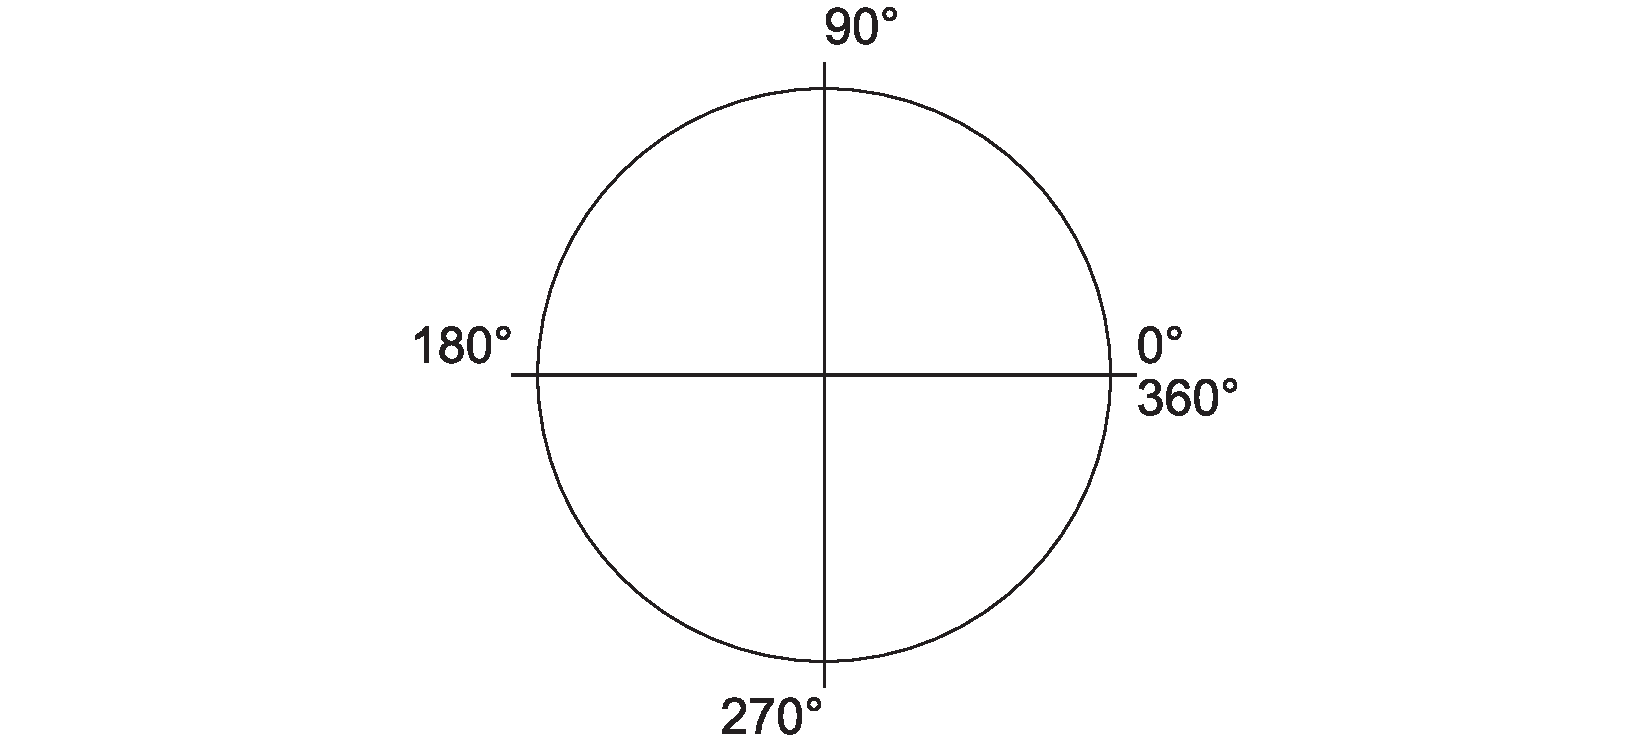
\includegraphics[width=\linewidth]{images/arcs_circle_degrees.pdf}%

Note that arcs of greater than 90 degrees are not rendered accurately, so, for the sake of
precision, they should be limited to a swing of 90 degrees or less. Further note that 4 arcs
may be stitched together to make a circle:
 
\begin{verbatim}
           dxfarc(small_square_tool_no,10,10,5,0,90);
           dxfarc(small_square_tool_no,10,10,5,90,180);
           dxfarc(small_square_tool_no,10,10,5,180,270);
           dxfarc(small_square_tool_no,10,10,5,270,360);
\end{verbatim}
 
A further refinement would be to connect multiple line segments/arcs into a larger polyline, 
but since most CAM tools implicitly join elements on import, that is not necessary.
 
There are three possible interactions for DXF elements and toolpaths:

\begin{itemize}
 \item describe the motion of the tool
 \item define a perimeter of an area which will be cut by a tool
 \item define a centerpoint for a specialty toolpath such as Drill or Keyhhole
\end{itemize}
 
\noindent and it is possible that multiple such elements could be instantiated for
a given toolpath.
 
\lstset{firstnumber=\thegcpscad}
\begin{writecode}{a}{gcodepreview.scad}{scad}
module dxfpl(tn,xbegin,ybegin,xend,yend) {
    dxfwrite(tn,"0");
    dxfwrite(tn,"LWPOLYLINE");
    dxfwrite(tn,"90");
    dxfwrite(tn,"2");
    dxfwrite(tn,"70");
    dxfwrite(tn,"0");
    dxfwrite(tn,"43");
    dxfwrite(tn,"0");
    dxfwrite(tn,"10");
    dxfwrite(tn,str(xbegin));
    dxfwrite(tn,"20");
    dxfwrite(tn,str(ybegin));
    dxfwrite(tn,"10");
    dxfwrite(tn,str(xend));
    dxfwrite(tn,"20");
    dxfwrite(tn,str(yend));
}

module dxfpolyline(tn,xbegin,ybegin,xend,yend) {
if (generatedxf == true) {
    dxfwriteone("0");
    dxfwriteone("LWPOLYLINE");
    dxfwriteone("90");
    dxfwriteone("2");
    dxfwriteone("70");
    dxfwriteone("0");
    dxfwriteone("43");
    dxfwriteone("0");
    dxfwriteone("10");
    dxfwriteone(str(xbegin));
    dxfwriteone("20");
    dxfwriteone(str(ybegin));
    dxfwriteone("10");
    dxfwriteone(str(xend));
    dxfwriteone("20");
    dxfwriteone(str(yend));
    dxfpl(tn,xbegin,ybegin,xend,yend);
    }
}

\end{writecode}
\addtocounter{gcpscad}{41}

As for other files, we have two versions, \DescribeRoutine{dxfa} and \DescribeRoutine{dxfarc}, 
one which accepts a \texttt{tn} (tool number), writing only to it, while a publicly facing version 
writes to the main DXF file \emph{and} writes to the specific DXF file for the specified tool.

\lstset{firstnumber=\thegcpscad}
\begin{writecode}{a}{gcodepreview.scad}{scad}
module dxfa(tn,xcenter,ycenter,radius,anglebegin,endangle) {
    dxfwrite(tn,"0");
    dxfwrite(tn,"ARC");
    dxfwrite(tn,"10");
    dxfwrite(tn,str(xcenter));
    dxfwrite(tn,"20");
    dxfwrite(tn,str(ycenter));
    dxfwrite(tn,"40");
    dxfwrite(tn,str(radius));
    dxfwrite(tn,"50");
    dxfwrite(tn,str(anglebegin));
    dxfwrite(tn,"51");
    dxfwrite(tn,str(endangle));
}

module dxfarc(tn,xcenter,ycenter,radius,anglebegin,endangle) {
if (generatedxf == true) {
    dxfwriteone("0");
    dxfwriteone("ARC");
    dxfwriteone("10");
    dxfwriteone(str(xcenter));
    dxfwriteone("20");
    dxfwriteone(str(ycenter));
    dxfwriteone("40");
    dxfwriteone(str(radius));
    dxfwriteone("50");
    dxfwriteone(str(anglebegin));
    dxfwriteone("51");
    dxfwriteone(str(endangle));
    dxfa(tn,xcenter,ycenter,radius,anglebegin,endangle);
    }
}

\end{writecode}
\addtocounter{gcpscad}{33}
 
The original implementation of polylines worked, but may be removed.
 
\lstset{firstnumber=\thegcpscad}
\begin{writecode}{a}{gcodepreview.scad}{scad}
module dxfbpl(tn,bx,by) {
    dxfwrite(tn,"0");
    dxfwrite(tn,"POLYLINE");
    dxfwrite(tn,"8");
    dxfwrite(tn,"default");
    dxfwrite(tn,"66");
    dxfwrite(tn,"1");
    dxfwrite(tn,"70");
    dxfwrite(tn,"0");
    dxfwrite(tn,"0");
    dxfwrite(tn,"VERTEX");
    dxfwrite(tn,"8");
    dxfwrite(tn,"default");
    dxfwrite(tn,"70");
    dxfwrite(tn,"32");
    dxfwrite(tn,"10");
    dxfwrite(tn,str(bx));
    dxfwrite(tn,"20");
    dxfwrite(tn,str(by));
}

module beginpolyline(bx,by,bz) {
if (generatedxf == true) {
    dxfwriteone("0");
    dxfwriteone("POLYLINE");
    dxfwriteone("8");
    dxfwriteone("default");
    dxfwriteone("66");
    dxfwriteone("1");
    dxfwriteone("70");
    dxfwriteone("0");
    dxfwriteone("0");
    dxfwriteone("VERTEX");
    dxfwriteone("8");
    dxfwriteone("default");
    dxfwriteone("70");
    dxfwriteone("32");
    dxfwriteone("10");
    dxfwriteone(str(bx));
    dxfwriteone("20");
    dxfwriteone(str(by));
    dxfbpl(current_tool(),bx,by);}
}

module dxfapl(tn,bx,by) {
    dxfwriteone("0");
    dxfwrite(tn,"VERTEX");
    dxfwrite(tn,"8");
    dxfwrite(tn,"default");
    dxfwrite(tn,"70");
    dxfwrite(tn,"32");
    dxfwrite(tn,"10");
    dxfwrite(tn,str(bx));
    dxfwrite(tn,"20");
    dxfwrite(tn,str(by));
}

module addpolyline(bx,by,bz) {
if (generatedxf == true) {
    dxfwrite(tn,"0");
    dxfwriteone("VERTEX");
    dxfwriteone("8");
    dxfwriteone("default");
    dxfwriteone("70");
    dxfwriteone("32");
    dxfwriteone("10");
    dxfwriteone(str(bx));
    dxfwriteone("20");
    dxfwriteone(str(by));
    dxfapl(current_tool(),bx,by);
    }
}

module dxfcpl(tn) {
    dxfwrite(tn,"0");
    dxfwrite(tn,"SEQEND");
}

module closepolyline() {
  if (generatedxf == true) {
    dxfwriteone("0");
    dxfwriteone("SEQEND");
    dxfcpl(current_tool());
  }
}

module writecomment(comment) {
  if (generategcode == true) {
    owritecomment(comment);
  }
}

\end{writecode}
\addtocounter{gcpscad}{92}
 
At the end of the project it will be necessary to close each file using the commands: 
\DescribeSubroutine{closegcodefile}{pclosegcodefile}, and
\DescribeRoutine{closedxffile}. %\DescribeRoutine{pclosesvgfile}
In some instances it will be necessary to write additional information,
depending on the file format.
 
\lstset{firstnumber=\thegcpy}
\begin{writecode}{a}{gcodepreview.py}{python}
def pclosegcodefile():
    f.close()

def pclosedxffile():
    dxf.close()

def pclosedxflgblfile():
    dxflgbl.close()

def pclosedxflgsqfile():
    dxflgsq.close()

def pclosedxflgVfile():
    dxflgV.close()

def pclosedxfsmblfile():
    dxfsmbl.close()

def pclosedxfsmsqfile():
    dxfsmsq.close()

def pclosedxfsmVfile():
    dxfsmV.close()

def pclosedxfDTfile():
    dxfDT.close()

def pclosedxfKHfile():
    dxfKH.close()

\end{writecode}
\addtocounter{gcpy}{30}
%def pclosesvgfile():
%    svg.close()
%

In addition to the Python forms, there will need to be matching OpenSCAD commands to call them:
\DescribeSubroutine{closegcodefile}{oclosegcodefile}, and 
\DescribeSubroutine{closedxffile}{oclosedxffile}.
%\DescribeSubroutine{oclosedxflgblfile}

\lstset{firstnumber=\thepyscad}
\begin{writecode}{a}{pygcodepreview.scad}{scad}
module oclosegcodefile() {
    pclosegcodefile();
}

module oclosedxffile() {
    pclosedxffile();
}

module oclosedxflgblfile() {
    pclosedxflgblfile();
}

module oclosedxflgsqfile() {
    pclosedxflgsqfile();
}

module oclosedxflgVfile() {
    pclosedxflgVfile();
}

module oclosedxfsmblfile() {
    pclosedxfsmblfile();
}

module oclosedxfsmsqfile() {
    pclosedxfsmsqfile();
}

module oclosedxfsmVfile() {
    pclosedxfsmVfile();
}

module oclosedxfDTfile() {
    pclosedxfDTfile();
}

module oclosedxfKHfile() {
    pclosedxfKHfile();
}

\end{writecode}
\addtocounter{pyscad}{40}
%module oclosesvgfile() {
%    pclosesvgfile();
%}
%

The commands: 
\DescribeRoutine{closegcodefile}, and
\DescribeRoutine{closedxffile}
are used to close the files at the end of a program. For efficiency, each references the command:
\DescribeRoutine{dxfpostamble}
which when called provides the boilerplate needed at the end of their respective files.

\lstset{firstnumber=\thegcpscad}
\begin{writecode}{a}{gcodepreview.scad}{scad}
module closegcodefile() {
  if (generategcode == true) {
    owriteone("M05");
    owriteone("M02");
    oclosegcodefile();
  }
}

module dxfpostamble(arg) {
    dxfwrite(arg,"0");
    dxfwrite(arg,"ENDSEC");
    dxfwrite(arg,"0");
    dxfwrite(arg,"EOF");
}

module closedxffile() {
  if (generatedxf == true) {
    dxfwriteone("0");
    dxfwriteone("ENDSEC");
    dxfwriteone("0");
    dxfwriteone("EOF");
    oclosedxffile();
    echo("CLOSING");
    if (large_ball_tool_no >  0) {    dxfpostamble(large_ball_tool_no);
      oclosedxflgblfile();
    } 
    if (large_square_tool_no >  0) {    dxfpostamble(large_square_tool_no);
      oclosedxflgsqfile();
    } 
    if (large_V_tool_no >  0) {    dxfpostamble(large_V_tool_no);
      oclosedxflgVfile();
    } 
    if (small_ball_tool_no >  0) {    dxfpostamble(small_ball_tool_no);
      oclosedxfsmblfile();
    } 
    if (small_square_tool_no >  0) {    dxfpostamble(small_square_tool_no);
      oclosedxfsmsqfile();
    } 
    if (small_V_tool_no >  0) {    dxfpostamble(small_V_tool_no);
      oclosedxfsmVfile();
    } 
    if (DT_tool_no >  0) {    dxfpostamble(DT_tool_no);
      oclosedxfDTfile();
    } 
    if (KH_tool_no >  0) {    dxfpostamble(KH_tool_no);
      oclosedxfKHfile();
    } 
  }
}

\end{writecode}
\addtocounter{gcpscad}{50}

%\lstset{firstnumber=\thegcpscad}
%\begin{writecode}{a}{gcodepreview.scad}{scad}
%module closesvgfile() {
%if (generatesvg == true) {
%    svgwriteone("</svg> ");
%    oclosesvgfile();
%    echo("CLOSING SVG");
%    }
%}
%
%\end{writecode}
%\addtocounter{gcpscad}{8}
 
\subsection{Movement and Cutting}

With all the scaffolding in place, it is possible to model the tool: 
\DescribeRoutine{otm}, (colors the tool model so as to differentiate cut areas)
and cutting: 
\DescribeRoutine{ocut}, 
as well as Rapid movements to position the tool to begin a cut:
\DescribeRoutine{orapid}%
which will also need to write out files which represent the desired machine motions.
 
\lstset{firstnumber=\thegcpscad}
\begin{writecode}{a}{gcodepreview.scad}{scad}
module otm(ex, ey, ez, r,g,b) {
color([r,g,b]) hull(){
    translate([xpos(), ypos(), zpos()]){
      select_tool(current_tool());
    }
    translate([ex, ey, ez]){
      select_tool(current_tool());
    }
  }
oset(ex, ey, ez);
}

module ocut(ex, ey, ez) {
  //color([0.2,1,0.2]) hull(){
  otm(ex, ey, ez, 0.2,1,0.2);
}

module orapid(ex, ey, ez) {
  //color([0.93,0,0]) hull(){
  otm(ex, ey, ez, 0.93,0,0);
}

module rapidbx(bx, by, bz, ex, ey, ez) {
  //    writeln("G0 X",bx," Y", by, "Z", bz);
  if (generategcode == true) {
    writecomment("rapid");
    owritesix("G0 X",str(ex)," Y", str(ey), " Z", str(ez));
  }
    orapid(ex, ey, ez);
}

module rapid(ex, ey, ez) {
  //    writeln("G0 X",bx," Y", by, "Z", bz);
  if (generategcode == true) {
      writecomment("rapid");
      owritesix("G0 X",str(ex)," Y", str(ey), " Z", str(ez));
  }
  orapid(ex, ey, ez);
}

module movetosafez() {
  //this should be move to retract height
  if (generategcode == true) {
      writecomment("Move to safe Z to avoid workholding");
      owriteone("G53G0Z-5.000");
  }
  orapid(getxpos(), getypos(), retractheight+55);
}

module begintoolpath(bx,by,bz) {
  if (generategcode == true) {
    writecomment("PREPOSITION FOR RAPID PLUNGE");
    owritefour("G0X", str(bx), "Y",str(by));
    owritetwo("Z", str(bz));
  }
  orapid(bx,by,bz);
}

module movetosafeheight() {
  //this should be move to machine position
  if (generategcode == true) {
  //    writecomment("PREPOSITION FOR RAPID PLUNGE");Z25.650
  //G1Z24.663F381.0 ,"F",str(plunge)
    if (zeroheight == "Top") {
      owritetwo("Z",str(retractheight));
    }
  }
    orapid(getxpos(), getypos(), retractheight+55);
}

module cutoneaxis_setfeed(axis,depth,feed) {
  if (generategcode == true) {
  //    writecomment("PREPOSITION FOR RAPID PLUNGE");Z25.650
  //G1Z24.663F381.0 ,"F",str(plunge) G1Z7.612F381.0
    if (zeroheight == "Top") {
      owritefive("G1",axis,str(depth),"F",str(feed));
    }
  }
  if (axis == "X") {setxpos(depth);
    ocut(depth, getypos(), getzpos());}
    if (axis == "Y") {setypos(depth);
      ocut(getxpos(), depth, getzpos());
    }
      if (axis == "Z") {setzpos(depth);
        ocut(getxpos(), getypos(), depth);
      }
}

module cut(ex, ey, ez) {
  //    writeln("G0 X",bx," Y", by, "Z", bz);
  if (generategcode == true) {
     owritesix("G1 X",str(ex)," Y", str(ey), " Z", str(ez));
  }
  //if (generatesvg == true) {
  //    owritesix("G1 X",str(ex)," Y", str(ey), " Z", str(ez));
  //    orapid(getxpos(), getypos(), retractheight+5);
  //    writesvgline(getxpos(),getypos(),ex,ey);
  //}
  ocut(ex, ey, ez);
}

module cutwithfeed(ex, ey, ez, feed) {
  //    writeln("G0 X",bx," Y", by, "Z", bz);
  if (generategcode == true) {
  //    writecomment("rapid");
    owriteeight("G1 X",str(ex)," Y", str(ey), " Z", str(ez),"F",str(feed));
  }
  ocut(ex, ey, ez);
}

module endtoolpath() {
  if (generategcode == true) {
  //Z31.750
  //    owriteone("G53G0Z-5.000");
    owritetwo("Z",str(retractheight));
  }
  orapid(getxpos(),getypos(),retractheight);
}

\end{writecode}
\addtocounter{gcpscad}{119}

\section{Cutting shapes, cut2Dshapes, and expansion}

Certain basic shapes (arcs, circles, rectangles), will be incorporated in the main code. 
Other shapes will be added to the additional/optional file, \texttt{cut2Dshapes.scad}
as they are developed, and of course the user is free to develop their own systems.
 
It is most expedient to test out new features in a new/separate file insofar as the 
file structures will allow (tool definitions for example will need to consolidated in 
\ref{subsubsec:toolchange}) which will need to be included in the projects which will 
make use of said features until such time as they are added into the main 
\texttt{gcodepreview.scad} file.

A basic requirement for two-dimensional regions will be to define them so as to cut them out.
Two different geometric treatments will be necessary: modeling the geometry which 
defines the region to be cut out (output as a DXF); and modeling the movement of the
tool, the toolpath which will be used in creating the 3D model and outputting the 
G-code.

In the TUG presentation/paper: \url{http://tug.org/TUGboat/tb40-2/tb125adams-3d.pdf}
a list of 2D shapes was put forward --- which of these will need to be created,
or if some more general solution will be put forward is uncertain. For the time
being, shapes will be implemented on an as-needed basis, as modified by the
interaction with the requirements of toolpaths.

\begin{figure}
\begin{outline}
\1 0
   \2 circle
   \2 ellipse (oval) (requires some sort of non-arc curve)
      \3 egg-shaped
   \2 annulus (one circle within another, forming  a ring)
   \2 superellipse (see astroid below)
\1 1
   \2 cone with rounded end (arc)—see also ``sector'' under 3 below
\1 2
   \2 semicircle/circular/half-circle segment (arc and a straight line); see also sector below
   \2 arch---curve possibly smoothly joining a  pair of straight lines with a flat bottom
   \2 lens/vesica piscis (two convex curves)
   \2 lune/crescent (one convex, one concave  curve)
   \2 heart (two curves)
   \2 tomoe (comma shape)---non-arc curves
\1 3
   \2 triangle
      \3 equilateral
      \3 isosceles
      \3 right triangle
      \3 scalene
   \2 (circular) sector (two straight edges, one convex arc)
      \3 quadrant (90\textdegree)
      \3 sextants (60\textdegree)
      \3 octants (45\textdegree)
   \2 deltoid curve (three concave arcs)
   \2  Reuleaux triangle (three convex arcs)
   \2 arbelos (one convex, two concave arcs)
   \2 two straight edges, one concave arc---an example is the hyperbolic sector\footnote{\url{en.wikipedia.org/wiki/Hyperbolic_sector} and
 \url{www.reddit.com/r/Geometry/comments/bkbzgh/is_there_a_name_for_a_3_pointed_figure_with_two}}
   \2 two convex, one concave arc
\1 4
   \2 rectangle (including square)
   \2 parallelogram
   \2 rhombus
   \2 trapezoid/trapezium
   \2 kite
   \2 ring/annulus segment (straight line, concave arc, straight line, convex arc)
   \2 astroid (four concave arcs)
   \2 salinon (four semicircles)
   \2 three straight lines and one concave arc
\end{outline}


  Is the list of shapes for which there are not widely
 known names interesting for its lack of notoriety?

\begin{itemize}
 \item two straight edges, one concave arc—oddly, an asymmetric form (hyperbolic sector) has a name,
       but not the symmetrical---while the colloquial/prosaic “arrowhead” was considered, it was
       rejected as being better applied to the shape below. (It’s also the shape used for the
       spaceship in the game Asteroids (or Hyperspace), but that  is potentially confusing with
       astroid.) At the  conference, Dr. Knuth suggested “dart” as a suitable term.
 \item two convex, one concave arc—with the above named, the term “arrowhead” is freed up to use
       as the name for this shape.
 \item three straight lines and one concave arc.
 \end{itemize}

 The first in particular is sorely needed for this project
 (it’s the result of inscribing a circle in a square or
 other regular geometric shape). Do these shapes
 have names in any other languages which might be
 used instead?
\end{figure}

The program Carbide Create has toolpath types and options which are as follows:

\begin{itemize}
 \item Contour --- No Offset --- the default, this is already supported in the existing code
 \item Contour --- Outside Offset
 \item Contour --- Inside Offset
 \item (Rectangular) Pocket --- such toolpaths/geometry should include the rounding of the tool 
       at the corners 
 \item Drill --- note that this is implemented as the plunging of a tool centered on a circle
                 and normally that circle is the same diameter as the tool which is used.
 \item Keyhole --- also beginning from a circle, a nice feature for this would be to 
                   include/model the areas which should be cleared for the sake of reducing wear
                   on the tool and ensuring chip clearance
\end{itemize}

 
Some further considerations:

\begin{itemize}
 \item relationship of geometry to toolpath --- arguably there should be an option for each
       toolpath (we will use Carbide Create as a reference implementation) which is to be 
       supported. Note that there are several possibilities: modeling the tool movement,
       describing the outline which the tool will cut, modeling a reference shape for the toolpath
 \item tool geometry --- it should be possible to include support for specialty tooling 
       such as dovetail cutters and to get an accurate 3D model, esp. for tooling which
       undercuts since they cannot be modeled in Carbide Create.
 \item feeds and speeds --- if outputting G-code it would be nice to be able to import feeds 
       and speeds from external files such as the .csv files used for user tool libraries in
       Carbide Create
 \item Starting and Max Depth --- are there CAD programs which will make use of Z-axis information 
       in a DXF? --- would it be possible/necessary to further differentiate the DXF geometry?
       (currently  written out separately for each toolpath in addition to one combined file)
\end{itemize}

\subsection{Arcs for toolpaths and DXFs}
 
A further consideration here is that G-code supports arcs in addition to the lines and
polylines already implemented. 

Implementing arcs wants at least the following options for quadrant and direction:
 
\begin{itemize}
\item cutarcNWCW --- cut the upper-left quadrant of a circle moving clockwise
\item cutarcNWCC --- upper-left quadrant counter-clockwise
\item cutarcNECW
\item cutarcNECC
\item cutarcSECW
\item cutarcSECC
\item cutarcNECW
\item cutarcNECC
\item cutcircleCW --- while it won’t matter for generating a DXF, when G-code is implemented
                      direction of cut will be a consideration for that
\item cutcircleCCdxf
\end{itemize}
 
It will be necessary to have two separate representations of arcs --- the DXF may be easily 
and directly supported with a single command, but representing the matching tool movement
in OpenSCAD will require a series of short line movements which approximate the arc. 
At this time, the current version of Carbide Create only imports circles in DXF as curves,
any other example is converted into polylines --- unfortunately, the implementation of this
is not such as would allow directly matching that representation. A work-around to import
a DXF as curves is to convert the arc into a reasonable number of line segments so as to
approximate the arc.
 
\begin{samepage}
Note that there are the following representations/interfaces for representing an arc:
 
\begin{itemize}
\item G-code --- G2 (clockwise) and G3 (counter-clockwise) arcs may be specified, and since 
      the endpoint is the positional requirement, it is most likely best to use the offset 
      to the center (I and J), rather than the radius parameter (K) \texttt{G2/3 ...} 
\item DXF --- \texttt{dxfarc(tn,xcenter,ycenter,radius,anglebegin,endangle)}
\item approximation of arc using lines (OpenSCAD) --- note that this may also be used 
      in DXF so as to sidestep the question of how many line segments there would be
      for a given arc representation 
\end{itemize}
\end{samepage}
 
Cutting the quadrant arcs will greatly simplify the calculation and interface for the modules.
A full set of 8 will be necessary, then circles may either be stitched together manually or
a pair of modules made for them.
 
At this time, despite what the module names imply (\texttt{cutarcNWCWdxf}, \&c.), only cutting  
and DXF generation is supported. Adding support for G-code will be done at a later time.
Since these modules will ultimately support G-code, the interface will assume the stored
\texttt{xpos} and \texttt{ypos} as the origin. Parameters which will need to be passed in are:
 
\begin{itemize}
 \item \texttt{tn}
 \item \texttt{ex}
 \item \texttt{ey}
 \item \texttt{ez} --- allowing a different Z position will make possible threading and
                       similar helical toolpaths
\item \texttt{xcenter} --- the center position will be specified as an absolute position
      which will require calculating the offset when it is used for G-code's \texttt{IJ},
      for which \texttt{xctr/yctr} are suggested 
\item \texttt{ycenter}
\item \texttt{radius} --- while this could be calculated, passing it in as a parameter
      is both convenient and acts as a check on the other parameters
\end{itemize}

Since OpenSCAD does not have an arc movement command it is necessary to iterate through a loop: \DescribeRoutine{arcloop} (clockwise), \DescribeRoutine{narcloop}
(counterclockwise) to handle the drawing and processing of the \texttt{cut()} toolpaths as 
short line segments which additionally affords a single point of control for adding additional
features such as allowing the depth to  vary as one cuts along an arc (two when the need to have 
a version which steps down):

\lstset{firstnumber=\thegcpscad}
\begin{writecode}{a}{gcodepreview.scad}{scad}
//!OpenSCAD

module arcloop(barc,earc, xcenter, ycenter, radius) {
  for (i = [barc : abs(1) : earc]) {
        cut(xcenter + radius * cos(i),
        ycenter + radius * sin(i),
        getzpos()-(gettzpos())
        );
    setxpos(xcenter + radius * cos(i));
    setypos(ycenter + radius * sin(i));
  }
}

module narcloop(barc,earc, xcenter, ycenter, radius) {
  for (i = [barc : -1 : earc]) {
        cut(xcenter + radius * cos(i),
        ycenter + radius * sin(i),
        getzpos()-(gettzpos())
        );
    setxpos(xcenter + radius * cos(i));
    setypos(ycenter + radius * sin(i));
  }
}

\end{writecode}
\addtocounter{gcpscad}{25}
 
The various textual versions are quite obvious:

\lstset{firstnumber=\thegcpscad}
\begin{writecode}{a}{gcodepreview.scad}{scad}
module cutarcNECCdxf(tn, ex, ey, ez, xcenter, ycenter, radius) {
  dxfarc(tn,xcenter,ycenter,radius,0,90);
  settzpos((getzpos()-ez)/90);
    arcloop(1,90, xcenter, ycenter, radius);
}

module cutarcNWCCdxf(tn, ex, ey, ez, xcenter, ycenter, radius) {
  dxfarc(tn,xcenter,ycenter,radius,90,180);
  settzpos((getzpos()-ez)/90);
    arcloop(91,180, xcenter, ycenter, radius);
}

module cutarcSWCCdxf(tn, ex, ey, ez, xcenter, ycenter, radius) {
  dxfarc(tn,xcenter,ycenter,radius,180,270);
  settzpos((getzpos()-ez)/90);
    arcloop(181,270, xcenter, ycenter, radius);
}

module cutarcSECCdxf(tn, ex, ey, ez, xcenter, ycenter, radius) {
  dxfarc(tn,xcenter,ycenter,radius,270,360);
  settzpos((getzpos()-ez)/90);
    arcloop(271,360, xcenter, ycenter, radius);
}

module cutarcNECWdxf(tn, ex, ey, ez, xcenter, ycenter, radius) {
  dxfarc(tn,xcenter,ycenter,radius,0,90);
  settzpos((getzpos()-ez)/90);
    narcloop(89,0, xcenter, ycenter, radius);
}

module cutarcSECWdxf(tn, ex, ey, ez, xcenter, ycenter, radius) {
  dxfarc(tn,xcenter,ycenter,radius,270,360);
  settzpos((getzpos()-ez)/90);
    narcloop(359,270, xcenter, ycenter, radius);
}

module cutarcSWCWdxf(tn, ex, ey, ez, xcenter, ycenter, radius) {
  dxfarc(tn,xcenter,ycenter,radius,180,270);
  settzpos((getzpos()-ez)/90);
    narcloop(269,180, xcenter, ycenter, radius);
}

module cutarcNWCWdxf(tn, ex, ey, ez, xcenter, ycenter, radius) {
  dxfarc(tn,xcenter,ycenter,radius,90,180);
  settzpos((getzpos()-ez)/90);
    narcloop(179,90, xcenter, ycenter, radius);
}

\end{writecode}
\addtocounter{gcpscad}{40}
 
\subsection{Keyhole toolpath and undercut tooling}
 
\label{subsec:keyholetoolpaths}
The first topologically unusual toolpath is \DescribeRoutine{keyhole toolpath} --- where 
other toolpaths have a 
direct correspondence between the associated geometry and the area cut, that Keyhole toolpaths
may be used with tooling which undercuts will result in the creation of two different physical
physical regions: the visible surface matching the union of the tool perimeter at the entry point
and the linear movement of the shaft and the larger region of the tool perimeter at the depth
which the tool is plunged to and moved along.
 
Tooling for such toolpaths is defined at paragraph~\ref{para:undercuttooling}

Due to the possibility of rotation, for the in-between positions there are more cases 
than one would think — for each quadrant there are the following possibilities:

\begin{itemize}
 \item one node on the clockwise side is outside of the quadrant
 \item two nodes on the clockwise side are outside of the quadrant
 \item all nodes are w/in the quadrant
 \item one node on the counter-clockwise side is outside of the quadrant
 \item two nodes on the counter-clockwise side are outside of the quadrant
\end{itemize}
 
Supporting all of these would require trigonometric comparisons in the If else blocks, 
so only the 4 quadrants, N, S, E, and W will be supported in the initial version. 
This will be done by wrapping the command with a version which only accepts those options: 

\lstset{firstnumber=\thegcpscad}
\begin{writecode}{a}{gcodepreview.scad}{scad}
module keyhole_toolpath(kh_tool_no, kh_start_depth, kh_max_depth, kht_angle, kh_length) {   
if (kht_angle == "N") {
  keyhole_toolpath_degrees(kh_tool_no, kh_start_depth, kh_max_depth, 90, kh_length);
    } else if (kht_angle == "S") {
  keyhole_toolpath_degrees(kh_tool_no, kh_start_depth, kh_max_depth, 270, kh_length);
    } else if (kht_angle == "E") {
  keyhole_toolpath_degrees(kh_tool_no, kh_start_depth, kh_max_depth, 0, kh_length);
    } else if (kht_angle == "W") {
  keyhole_toolpath_degrees(kh_tool_no, kh_start_depth, kh_max_depth, 180, kh_length);
    }
}

\end{writecode}
\addtocounter{gcpscad}{12}
 
The original version of the command, \DescribeRoutine{keyhole toolpath degrees} retains 
an interface which allows calling it for arbitrary beginning and ending points of an arc. 
Note that code is still present for the partial calculation of one quadrant (for the case of 
all nodes within the quadrant).

The first task is to place a circle at the origin which is invariant of angle:
 
\lstset{firstnumber=\thegcpscad}
\begin{writecode}{a}{gcodepreview.scad}{scad}
module keyhole_toolpath_degrees(kh_tool_no, kh_start_depth, kh_max_depth, kh_angle, kh_length) {
dxfarc(KH_tool_no,getxpos(),getypos(),tool_diameter(KH_tool_no, (kh_max_depth+4.36))/2,0,90);
dxfarc(KH_tool_no,getxpos(),getypos(),tool_diameter(KH_tool_no, (kh_max_depth+4.36))/2,90,180);
dxfarc(KH_tool_no,getxpos(),getypos(),tool_diameter(KH_tool_no, (kh_max_depth+4.36))/2,180,270);
dxfarc(KH_tool_no,getxpos(),getypos(),tool_diameter(KH_tool_no, (kh_max_depth+4.36))/2,270,360);

\end{writecode}
\addtocounter{gcpscad}{6}

Then it will be necessary to test for each possible case in a series of If Else blocks:
 
\lstset{firstnumber=\thegcpscad}
\begin{writecode}{a}{gcodepreview.scad}{scad}
  if (kh_angle == 0) {
dxfarc(KH_tool_no,getxpos(),getypos(),tool_diameter(KH_tool_no, (kh_max_depth))/2,180,270);
dxfarc(KH_tool_no,getxpos(),getypos(),tool_diameter(KH_tool_no, (kh_max_depth))/2,90,180);
dxfarc(KH_tool_no,getxpos(),getypos(),tool_diameter(KH_tool_no, (kh_max_depth))/2,asin((tool_diameter(KH_tool_no, (kh_max_depth+4.36))/2)/(tool_diameter(KH_tool_no, (kh_max_depth))/2)),90);
dxfarc(KH_tool_no,getxpos(),getypos(),tool_diameter(KH_tool_no, (kh_max_depth))/2,270,360-asin((tool_diameter(KH_tool_no, (kh_max_depth+4.36))/2)/(tool_diameter(KH_tool_no, (kh_max_depth))/2)));
dxfarc(KH_tool_no,getxpos()+kh_length,getypos(),tool_diameter(KH_tool_no, (kh_max_depth+4.36))/2,0,90);
dxfarc(KH_tool_no,getxpos()+kh_length,getypos(),tool_diameter(KH_tool_no, (kh_max_depth+4.36))/2,270,360);
dxfpolyline(KH_tool_no, getxpos()+sqrt((tool_diameter(KH_tool_no, (kh_max_depth))/2)^2-(tool_diameter(KH_tool_no, (kh_max_depth+4.36))/2)^2), getypos()+tool_diameter(KH_tool_no, (kh_max_depth+4.36))/2, getxpos()+kh_length, getypos()+tool_diameter(KH_tool_no, (kh_max_depth+4.36))/2);
dxfpolyline(KH_tool_no, getxpos()+sqrt((tool_diameter(KH_tool_no, (kh_max_depth))/2)^2-(tool_diameter(KH_tool_no, (kh_max_depth+4.36))/2)^2), getypos()-tool_diameter(KH_tool_no, (kh_max_depth+4.36))/2, getxpos()+kh_length, getypos()-tool_diameter(KH_tool_no, (kh_max_depth+4.36))/2);
dxfpolyline(KH_tool_no,getxpos(),getypos(),getxpos()+kh_length,getypos());
cutwithfeed(getxpos()+kh_length,getypos(),-kh_max_depth,feed);
setxpos(getxpos()-kh_length);
  } else if (kh_angle > 0 && kh_angle < 90) {
echo(kh_angle);
  dxfarc(KH_tool_no,getxpos(),getypos(),tool_diameter(KH_tool_no, (kh_max_depth))/2,90+kh_angle,180+kh_angle);
  dxfarc(KH_tool_no,getxpos(),getypos(),tool_diameter(KH_tool_no, (kh_max_depth))/2,180+kh_angle,270+kh_angle);
dxfarc(KH_tool_no,getxpos(),getypos(),tool_diameter(KH_tool_no, (kh_max_depth))/2,kh_angle+asin((tool_diameter(KH_tool_no, (kh_max_depth+4.36))/2)/(tool_diameter(KH_tool_no, (kh_max_depth))/2)),90+kh_angle);
dxfarc(KH_tool_no,getxpos(),getypos(),tool_diameter(KH_tool_no, (kh_max_depth))/2,270+kh_angle,360+kh_angle-asin((tool_diameter(KH_tool_no, (kh_max_depth+4.36))/2)/(tool_diameter(KH_tool_no, (kh_max_depth))/2)));
dxfarc(KH_tool_no,
  getxpos()+(kh_length*cos(kh_angle)),
  getypos()+(kh_length*sin(kh_angle)),tool_diameter(KH_tool_no, (kh_max_depth+4.36))/2,0+kh_angle,90+kh_angle);
dxfarc(KH_tool_no,getxpos()+(kh_length*cos(kh_angle)),getypos()+(kh_length*sin(kh_angle)),tool_diameter(KH_tool_no, (kh_max_depth+4.36))/2,270+kh_angle,360+kh_angle);
dxfpolyline(KH_tool_no,
 getxpos()+tool_diameter(KH_tool_no, (kh_max_depth))/2*cos(kh_angle+asin((tool_diameter(KH_tool_no, (kh_max_depth+4.36))/2)/(tool_diameter(KH_tool_no, (kh_max_depth))/2))),
 getypos()+tool_diameter(KH_tool_no, (kh_max_depth))/2*sin(kh_angle+asin((tool_diameter(KH_tool_no, (kh_max_depth+4.36))/2)/(tool_diameter(KH_tool_no, (kh_max_depth))/2))),
 getxpos()+(kh_length*cos(kh_angle))-((tool_diameter(KH_tool_no, (kh_max_depth+4.36))/2)*sin(kh_angle)),
 getypos()+(kh_length*sin(kh_angle))+((tool_diameter(KH_tool_no, (kh_max_depth+4.36))/2)*cos(kh_angle)));
echo("a",tool_diameter(KH_tool_no, (kh_max_depth+4.36))/2);
echo("c",tool_diameter(KH_tool_no, (kh_max_depth))/2);
echo("Aangle",asin((tool_diameter(KH_tool_no, (kh_max_depth+4.36))/2)/(tool_diameter(KH_tool_no, (kh_max_depth))/2)));
echo(kh_angle);
 cutwithfeed(getxpos()+(kh_length*cos(kh_angle)),getypos()+(kh_length*sin(kh_angle)),-kh_max_depth,feed);
 setxpos(getxpos()-(kh_length*cos(kh_angle)));
 setypos(getypos()-(kh_length*sin(kh_angle)));
  } else if (kh_angle == 90) {
dxfarc(KH_tool_no,getxpos(),getypos(),tool_diameter(KH_tool_no, (kh_max_depth))/2,180,270);
dxfarc(KH_tool_no,getxpos(),getypos(),tool_diameter(KH_tool_no, (kh_max_depth))/2,270,360);
dxfarc(KH_tool_no,getxpos(),getypos(),tool_diameter(KH_tool_no, (kh_max_depth))/2,0,90-asin(
    (tool_diameter(KH_tool_no, (kh_max_depth+4.36))/2)/(tool_diameter(KH_tool_no, (kh_max_depth))/2)));
dxfarc(KH_tool_no,getxpos(),getypos(),tool_diameter(KH_tool_no, (kh_max_depth))/2,90+asin(
    (tool_diameter(KH_tool_no, (kh_max_depth+4.36))/2)/(tool_diameter(KH_tool_no, (kh_max_depth))/2)),180);
 dxfpolyline(KH_tool_no,getxpos(),getypos(),getxpos(),getypos()+kh_length);
dxfarc(KH_tool_no,getxpos(),getypos()+kh_length,tool_diameter(KH_tool_no, (kh_max_depth+4.36))/2,0,90);
dxfarc(KH_tool_no,getxpos(),getypos()+kh_length,tool_diameter(KH_tool_no, (kh_max_depth+4.36))/2,90,180);
 dxfpolyline(KH_tool_no,getxpos()+tool_diameter(KH_tool_no, (kh_max_depth+4.36))/2,getypos()+sqrt((tool_diameter(KH_tool_no, (kh_max_depth))/2)^2-(tool_diameter(KH_tool_no, (kh_max_depth+4.36))/2)^2),getxpos()+tool_diameter(KH_tool_no, (kh_max_depth+4.36))/2,getypos()+kh_length);
 dxfpolyline(KH_tool_no,getxpos()-tool_diameter(KH_tool_no, (kh_max_depth+4.36))/2,getypos()+sqrt((tool_diameter(KH_tool_no, (kh_max_depth))/2)^2-(tool_diameter(KH_tool_no, (kh_max_depth+4.36))/2)^2),getxpos()-tool_diameter(KH_tool_no, (kh_max_depth+4.36))/2,getypos()+kh_length);
 cutwithfeed(getxpos(),getypos()+kh_length,-kh_max_depth,feed);
 setypos(getypos()-kh_length);
  } else if (kh_angle == 180) {
dxfarc(KH_tool_no,getxpos(),getypos(),tool_diameter(KH_tool_no, (kh_max_depth))/2,0,90);
dxfarc(KH_tool_no,getxpos(),getypos(),tool_diameter(KH_tool_no, (kh_max_depth))/2,270,360);
dxfarc(KH_tool_no,getxpos(),getypos(),tool_diameter(KH_tool_no, (kh_max_depth))/2,90,180-asin((tool_diameter(KH_tool_no, (kh_max_depth+4.36))/2)/(tool_diameter(KH_tool_no, (kh_max_depth))/2)));
dxfarc(KH_tool_no,getxpos(),getypos(),tool_diameter(KH_tool_no, (kh_max_depth))/2,180+asin((tool_diameter(KH_tool_no, (kh_max_depth+4.36))/2)/(tool_diameter(KH_tool_no, (kh_max_depth))/2)),270);
dxfarc(KH_tool_no,getxpos()-kh_length,getypos(),tool_diameter(KH_tool_no, (kh_max_depth+4.36))/2,90,180);
dxfarc(KH_tool_no,getxpos()-kh_length,getypos(),tool_diameter(KH_tool_no, (kh_max_depth+4.36))/2,180,270);
dxfpolyline(KH_tool_no,
 getxpos()-sqrt((tool_diameter(KH_tool_no, (kh_max_depth))/2)^2-(tool_diameter(KH_tool_no, (kh_max_depth+4.36))/2)^2),
 getypos()+tool_diameter(KH_tool_no, (kh_max_depth+4.36))/2,
 getxpos()-kh_length,
 getypos()+tool_diameter(KH_tool_no, (kh_max_depth+4.36))/2);
dxfpolyline(KH_tool_no,
 getxpos()-sqrt((tool_diameter(KH_tool_no, (kh_max_depth))/2)^2-(tool_diameter(KH_tool_no, (kh_max_depth+4.36))/2)^2),
 getypos()-tool_diameter(KH_tool_no, (kh_max_depth+4.36))/2,
 getxpos()-kh_length,
 getypos()-tool_diameter(KH_tool_no, (kh_max_depth+4.36))/2);
 dxfpolyline(KH_tool_no,getxpos(),getypos(),getxpos()-kh_length,getypos());
 cutwithfeed(getxpos()-kh_length,getypos(),-kh_max_depth,feed);
 setxpos(getxpos()+kh_length);
  } else if (kh_angle == 270) {
dxfarc(KH_tool_no,getxpos(),getypos(),tool_diameter(KH_tool_no, (kh_max_depth))/2,0,90);
dxfarc(KH_tool_no,getxpos(),getypos(),tool_diameter(KH_tool_no, (kh_max_depth))/2,90,180);
dxfarc(KH_tool_no,getxpos(),getypos(),tool_diameter(KH_tool_no, (kh_max_depth))/2,270+asin((tool_diameter(KH_tool_no, (kh_max_depth+4.36))/2)/(tool_diameter(KH_tool_no, (kh_max_depth))/2)),360);
dxfarc(KH_tool_no,getxpos(),getypos(),tool_diameter(KH_tool_no, (kh_max_depth))/2,180, 270-asin((tool_diameter(KH_tool_no, (kh_max_depth+4.36))/2)/(tool_diameter(KH_tool_no, (kh_max_depth))/2)));
dxfarc(KH_tool_no,getxpos(),getypos()-kh_length,tool_diameter(KH_tool_no, (kh_max_depth+4.36))/2,180,270);
dxfarc(KH_tool_no,getxpos(),getypos()-kh_length,tool_diameter(KH_tool_no, (kh_max_depth+4.36))/2,270,360);
 dxfpolyline(KH_tool_no,getxpos()+tool_diameter(KH_tool_no, (kh_max_depth+4.36))/2,getypos()-sqrt((tool_diameter(KH_tool_no, (kh_max_depth))/2)^2-(tool_diameter(KH_tool_no, (kh_max_depth+4.36))/2)^2),getxpos()+tool_diameter(KH_tool_no, (kh_max_depth+4.36))/2,getypos()-kh_length);
 dxfpolyline(KH_tool_no,getxpos()-tool_diameter(KH_tool_no, (kh_max_depth+4.36))/2,getypos()-sqrt((tool_diameter(KH_tool_no, (kh_max_depth))/2)^2-(tool_diameter(KH_tool_no, (kh_max_depth+4.36))/2)^2),getxpos()-tool_diameter(KH_tool_no, (kh_max_depth+4.36))/2,getypos()-kh_length);
 dxfpolyline(KH_tool_no,getxpos(),getypos(),getxpos(),getypos()-kh_length);
 cutwithfeed(getxpos(),getypos()-kh_length,-kh_max_depth,feed);
 setypos(getypos()+kh_length);
  }
}

\end{writecode}
\addtocounter{gcpscad}{91}
 
\subsection{Shapes and tool movement}
 
The majority of commands will be more general, focusing on tooling which is generally
supported by this library, moving in lines and arcs so as to describe shapes which
lend themselves to representation with those tool and which match up with both
toolpaths and supported geometry in Carbide Create, and the usage requirements of
the typical user.

\subsubsection{Generalized commands and cuts}

The first consideration is a naming convention which will allow a generalized set of associated
commands to be defined. The initial version will only create OpenSCAD commands for 3D modeling
and write out matching DXF files. At a later time this will be extended with G-code support.
 
\paragraph{begincutdxf}
 
The first command, \DescribeRoutine{begincutdxf} will need to allow the machine to rapid to 
the beginning point of the cut and then rapid down to the surface of the stock, and then 
plunge down to the depth of the cut. The implementation will need to allow for a hook where 
the Depth per Pass is applied to the plunge operation so that multiple passes are made.

The first module will ensure that the tool is safely up above
the stock and will rapid to the position specified at the retract height (moving to that 
position as an initial step, then will \texttt{cutwithfeed} to the specified position
at the specified feed rate. Despite \texttt{dxf} being included in the filename no change
is made to the dxf file at this time, this simply indicates that this file is preparatory to
the use of \DescribeRoutine{continuecutdxf}.

\lstset{firstnumber=\thegcpscad}
\begin{writecode}{a}{gcodepreview.scad}{scad}
module begincutdxf(rh, ex, ey, ez, fr) {
  rapid(getxpos(),getypos(),rh);
  cutwithfeed(ex,ey,ez,fr);
}

\end{writecode}
\addtocounter{gcpscad}{5}
 
\lstset{firstnumber=\thegcpscad}
\begin{writecode}{a}{gcodepreview.scad}{scad}
module continuecutdxf(ex, ey, ez, fr) {
  cutwithfeed(ex,ey,ez,fr);
}

\end{writecode}
\addtocounter{gcpscad}{4}

\paragraph{Rectangles}

Cutting rectangles while writing out their perimeter in the DXF files (so that they may
be assigned a matching toolpath in a traditional CAM program upon import) will require
the origin coordinates, height and width and depth of the pocket, and the tool \# so
that the corners may have a radius equal to the tool which is used. Whether a given module
is an interior pocket or an outline (interior or exterior) will be determined by the
specifics of the module and its usage/positioning, with \texttt{outline} being added to 
those modules which cut perimeter.

A further consideration is that cut orientation as an option should be accounted for
if writing out G-code, as well as stepover, and the nature of initial
entry (whether ramping in would be implemented, and if so, at what angle). Advanced 
toolpath strategies such as trochoidal milling could also be implemented.

Th routine \DescribeRoutine{cutrectangledxf}%
cuts the outline of a rectangle creating sharp corners. Note that the initial 
version would work as a beginning point for vertical cutting if the \texttt{hull()} operation 
was removed and the loop was uncommented:
 
\lstset{firstnumber=\thegcpscad}
\begin{writecode}{a}{gcodepreview.scad}{scad}
module cutrectangledxf(bx, by, bz, rwidth, rheight, rdepth, rtn) {//passes
  movetosafez();
  hull(){
    //  for (i = [0 : abs(1) : passes]) {
    //      rapid(bx+tool_radius(rtn)+i*(rwidth-tool_diameter(current_tool()))/passes,bx+tool_radius(rtn),1);
    //      cutwithfeed(bx+tool_radius(rtn)+i*(rwidth-tool_diameter(current_tool()))/passes,by+tool_radius(rtn),bz-rdepth,feed);
    //      cutwithfeed(bx+tool_radius(rtn)+i*(rwidth-tool_diameter(current_tool()))/passes,by+rheight-tool_radius(rtn),bz-rdepth,feed);
  
    cutwithfeed(bx+tool_radius(rtn),by+tool_radius(rtn),bz-rdepth,feed);
    cutwithfeed(bx+rwidth-tool_radius(rtn),by+tool_radius(rtn),bz-rdepth,feed);
    cutwithfeed(bx+rwidth-tool_radius(rtn),by+rheight-tool_radius(rtn),bz-rdepth,feed);
    cutwithfeed(bx+tool_radius(rtn),by+rheight-tool_radius(rtn),bz-rdepth,feed);
  }
  //dxfarc(tn,xcenter,ycenter,radius,anglebegin,endangle)
  dxfarc(rtn,bx+tool_radius(rtn),by+tool_radius(rtn),tool_radius(rtn),180,270);
  //dxfpolyline(tn,xbegin,ybegin,xend,yend)
  dxfpolyline(rtn,bx,by+tool_radius(rtn),bx,by+rheight-tool_radius(rtn));
  dxfarc(rtn,bx+tool_radius(rtn),by+rheight-tool_radius(rtn),tool_radius(rtn),90,180);
  dxfpolyline(rtn,bx+tool_radius(rtn),by+rheight,bx+rwidth-tool_radius(rtn),by+rheight);
  dxfarc(rtn,bx+rwidth-tool_radius(rtn),by+rheight-tool_radius(rtn),tool_radius(rtn),0,90);
  dxfpolyline(rtn,bx+rwidth,by+rheight-tool_radius(rtn),bx+rwidth,by+tool_radius(rtn));
  dxfarc(rtn,bx+rwidth-tool_radius(rtn),by+tool_radius(rtn),tool_radius(rtn),270,360);
  dxfpolyline(rtn,bx+rwidth-tool_radius(rtn),by,bx+tool_radius(rtn),by);
}

\end{writecode}
\addtocounter{gcpscad}{25}

A matching command: \DescribeRoutine{cutrectangleoutlinedxf}%
cuts the outline of a rounded rectangle and is a simplification of the above:

\lstset{firstnumber=\thegcpscad}
\begin{writecode}{a}{gcodepreview.scad}{scad}
module cutrectangleoutlinedxf(bx, by, bz, rwidth, rheight, rdepth, rtn) {//passes
  movetosafez();
  cutwithfeed(bx+tool_radius(rtn),by+tool_radius(rtn),bz-rdepth,feed);
  cutwithfeed(bx+rwidth-tool_radius(rtn),by+tool_radius(rtn),bz-rdepth,feed);
  cutwithfeed(bx+rwidth-tool_radius(rtn),by+rheight-tool_radius(rtn),bz-rdepth,feed);
  cutwithfeed(bx+tool_radius(rtn),by+rheight-tool_radius(rtn),bz-rdepth,feed);
  dxfarc(rtn,bx+tool_radius(rtn),by+tool_radius(rtn),tool_radius(rtn),180,270);
  dxfpolyline(rtn,bx,by+tool_radius(rtn),bx,by+rheight-tool_radius(rtn));
  dxfarc(rtn,bx+tool_radius(rtn),by+rheight-tool_radius(rtn),tool_radius(rtn),90,180);
  dxfpolyline(rtn,bx+tool_radius(rtn),by+rheight,bx+rwidth-tool_radius(rtn),by+rheight);
  dxfarc(rtn,bx+rwidth-tool_radius(rtn),by+rheight-tool_radius(rtn),tool_radius(rtn),0,90);
  dxfpolyline(rtn,bx+rwidth,by+rheight-tool_radius(rtn),bx+rwidth,by+tool_radius(rtn));
  dxfarc(rtn,bx+rwidth-tool_radius(rtn),by+tool_radius(rtn),tool_radius(rtn),270,360);
  dxfpolyline(rtn,bx+rwidth-tool_radius(rtn),by,bx+tool_radius(rtn),by);
}

\end{writecode}
\addtocounter{gcpscad}{16}

Which suggests a further command, \DescribeRoutine{rectangleoutlinedxf}
for simply adding a rectangle (a potential use of
which would be in Job Setup to add the stock outline to DXFs to assist in registration 
of jobs with multiple tools):

\lstset{firstnumber=\thegcpscad}
\begin{writecode}{a}{gcodepreview.scad}{scad}
module rectangleoutlinedxf(bx, by, bz, rwidth, rheight, rtn) {
  dxfpolyline(rtn,bx,by,bx,by+rheight);
  dxfpolyline(rtn,bx,by+rheight,bx+rwidth,by+rheight);
  dxfpolyline(rtn,bx+rwidth,by+rheight,bx+rwidth,by);
  dxfpolyline(rtn,bx+rwidth,by,bx,by);
}

\end{writecode}
\addtocounter{gcpscad}{7}

\noindent the initial section performs the cutting operation for the 3D preview while the 
latter section writes out the outline to the DXF files.

A variant of the  cutting version of that file, \DescribeRoutine{cutoutrectangledxf} 
will cut to the outside:

\lstset{firstnumber=\thegcpscad}
\begin{writecode}{a}{gcodepreview.scad}{scad}
module cutoutrectangledxf(bx, by, bz, rwidth, rheight, rdepth, rtn) {
  movetosafez();
  cutwithfeed(bx-tool_radius(rtn),by-tool_radius(rtn),bz-rdepth,feed);
  cutwithfeed(bx+rwidth+tool_radius(rtn),by-tool_radius(rtn),bz-rdepth,feed);
  cutwithfeed(bx+rwidth+tool_radius(rtn),by+rheight+tool_radius(rtn),bz-rdepth,feed);
  cutwithfeed(bx-tool_radius(rtn),by+rheight+tool_radius(rtn),bz-rdepth,feed);
  cutwithfeed(bx-tool_radius(rtn),by-tool_radius(rtn),bz-rdepth,feed);
  dxfpolyline(rtn,bx,by,bx,by+rheight);
  dxfpolyline(rtn,bx,by+rheight,bx+rwidth,by+rheight);
  dxfpolyline(rtn,bx+rwidth,by+rheight,bx+rwidth,by);
  dxfpolyline(rtn,bx+rwidth,by,bx,by);
}

\end{writecode}
\addtocounter{gcpscad}{13}

\subsection{Expansion}

The balance of shapes will go into \texttt{cut2Dshapes.scad} and of course it will be 
possible to create additional files for specific purposes.

\lstset{firstnumber=1}
\begin{writecode}{w}{cut2Dshapes.scad}{scad}
//!OpenSCAD

\end{writecode}
\addtocounter{cuttwod}{2}

\section{gcodepreviewtemplate.scad}

The commands may then be put together using a template which will ensure that
the various files are used/included as necessary, that files are opened before
being written to, and that they are closed at the end.

\lstset{firstnumber=1}%\thegcptmpl}
\begin{writecode}{w}{gcodepreviewtemplate.scad}{scad}
//!OpenSCAD

use <gcodepreview.py>;
use <pygcodepreview.scad>;
include <gcodepreview.scad>;

$fa = 2;
$fs = 0.125;

/* [Export] */
Base_filename = "export"; 

/* [Export] */
generatedxf = true; 

/* [Export] */
generategcode = true; 

///* [Export] */
//generatesvg = false; 

/* [CAM] */
toolradius = 1.5875;

/* [CAM] */
large_ball_tool_no = 0; // [0:0,111:111,101:101,202:202]

/* [CAM] */
large_square_tool_no = 0; // [0:0,112:112,102:102,201:201]

/* [CAM] */
large_V_tool_no = 0; // [0:0,301:301,690:690]

/* [CAM] */
small_ball_tool_no = 0; // [0:0,121:121,111:111,101:101]

/* [CAM] */
small_square_tool_no = 102; // [0:0,122:122,112:112,102:102]

/* [CAM] */
small_V_tool_no = 0; // [0:0,390:390,301:301]

/* [CAM] */
KH_tool_no = 0; // [0:0,375:375]

/* [CAM] */
DT_tool_no = 0; // [0:0,814:814]

/* [Feeds and Speeds] */
plunge = 100;

/* [Feeds and Speeds] */
feed = 400;

/* [Feeds and Speeds] */
speed = 16000;

/* [Feeds and Speeds] */
square_ratio = 1.0; // [0.25:2]

/* [Feeds and Speeds] */
small_V_ratio = 0.75; // [0.25:2]

/* [Feeds and Speeds] */
large_V_ratio = 0.875; // [0.25:2]

/* [Stock] */
stocklength = 219;

/* [Stock] */
stockwidth = 150;

/* [Stock] */
stockthickness = 8.35;

/* [Stock] */
zeroheight = "Top"; // [Top, Bottom]

/* [Stock] */
stockorigin = "Center"; // [Lower-Left, Center-Left, Top-Left, Center]

/* [Stock] */
retractheight = 9;

filename_gcode = str(Base_filename, ".nc");
filename_dxf = str(Base_filename);
//filename_svg = str(Base_filename, ".svg");

opengcodefile(filename_gcode);
opendxffile(filename_dxf);

difference() {
setupstock(stocklength, stockwidth, stockthickness, zeroheight, stockorigin);

movetosafez();

toolchange(small_square_tool_no,speed * square_ratio);

begintoolpath(0,0,0.25);
beginpolyline(0,0,0.25);

cutoneaxis_setfeed("Z",0,plunge*square_ratio);

cutwithfeed(stocklength/2,stockwidth/2,-stockthickness,feed);
addpolyline(stocklength/2,stockwidth/2,-stockthickness);

endtoolpath();
closepolyline();
}

closegcodefile();
closedxffile();
\end{writecode}
\addtocounter{gcptmpl}{112}
 
\section{Future}

\subsection{Images}

Would it be helpful to re-create code algorithms/sections using OpenSCAD Graph Editor 
so as to represent/illustrate the program?

\subsection{Generalized DXF creation}

Generalize the creation of DXFs based on the projection() of a toolpath?

\subsection{Import G-code}

Use a tool to read in a G-code file, then create a 3D model which would serve as a preview of the cut?

\begin{itemize}
\item \url{https://stackoverflow.com/questions/34638372/simple-python-program-to-read-gcode-file}
\item \url{https://pypi.org/project/gcodeparser/}
\item \url{https://github.com/fragmuffin/pygcode/wiki}
\end{itemize} 
 
\subsection{Bézier curves in 2 dimensions}

Take a Bézier curve definition and approximate it as arcs and write them into a DXF?

\url{https://pomax.github.io/bezierinfo/}

c.f., \url{https://linuxcnc.org/docs/html/gcode/g-code.html#gcode:g5}

%There is Bernstein polynomial equation which is similar to calculating like $(a+b)^2 ....$ or up to $(a+b)^n$ where $n$ is the degree of polynomial.
%
%So how do you calculate $(a+b)^2$ or for that matter to any polynomial degree $n$
%
%an integer $i => 0 to n$ calculates each term of the above equation
%
%$n!/(i! * (n-i)!)*a^i*b^(n-i)$  where $n!$ means factorial of $n$ --equation 1
%substituting $a=t$ and $b=(1-t)$
%where $t$ is a parameter which goes from $0 ->1$ and you can have any numbers within that range
%
%in bezier the degree of the curve is 1 less than the control points e.g. if you have 10 control points the polynomial degree will be 9.
%
%so finally equation for bezier is:
%
%$sum(p[i]*n!/(i! * (n-i)!)*t^i*(1-t)^(n-i))$ where $p[i]$ is the $i$th control point
%
%my simple 6 lines function for bezier curve is following:
%
%\begin{verbatim}
%def bezier(p,s=10):
%  r  '''
%    bezier curve defined by points 'p' and number of segments 's'
%    '''
%    p=a_(p)
%    n=len(p)
%    k=n-1
%    f=[[p[i]*comb(k,i)*u**i*(1-u)**(k-i) for i in range(n)]
%       for u in linspace(0,1,s)]    
%    p1=l_(a_([p.sum(0) for p in a_(f)]))
%    return p1
%\end{verbatim}    

\subsection{Bézier curves in 3 dimensions}
 
One question is how many Bézier curves would it be necessary to have to define a surface
in 3 dimensions. Attributes for this which are desirable/necessary:

\begin{itemize}
\item concise --- a given Bézier curve should be represented by just the point coordinates, 
      so two on-curve points, two off-curve points, each with a pair of coordinates
\item For a given shape/region it will need to be possible to have a matching definition 
      exactly match up with it so that one could piece together a larger more complex shape 
      from smaller/simpler regions
\item similarly it will be necessary for it to be possible to sub-divide a defined region --- 
      for example it should be possible if one had 4 adjacent regions, then the four quadrants 
      at the intersection of the four regions could be used to construct a new region --- is it
      possible to derive a new Bézier curve from half of two other curves?
\end{itemize}

\begin{samepage}
For the three planes:

\begin{itemize}
 \item XY
 \item XZ
 \item ZY
\end{itemize}
 
\noindent it should be possible to have three Bézier curves (left-most/right-most or front-back or 
top/bottom for two, and a mid-line for the third), so a region which can be so represented would 
be definable by:
 
\begin{verbatim}
3 planes * 3 Béziers * (2 on-curve + 2 off-curve points) == 36 coordinate pairs
\end{verbatim}
\end{samepage}
 
\noindent which is a marked contrast to representations such as:
 
\url{https://github.com/DavidPhillipOster/Teapot}

\noindent and regions which could not be so represented could be sub-divided until the 
representation is workable.

Or, it may be that fewer (only two?) curves are needed:

\noindent\includegraphics[width=\linewidth]{images/Screenshot 2024-08-11 at 6.55.26 PM.png}

\url{https://pages.mtu.edu/~shene/COURSES/cs3621/NOTES/notes.html}

\section{Other Resources}
 
Holidays are from \url{https://nationaltoday.com/}

%This document was re-worked per: \url{https://tex.stackexchange.com/questions/47237/different-approach-to-literate-programming-for-latex}
 
\bibliographystyle{alpha}

\begin{thebibliography}{PractShopMath}

\bibitem[ConstGeom]{WALMSLEY81}
Walmsley, Brian. \emph{Construction Geometry}. 2d ed., Centennial College Press, 1981.
 
\bibitem[MkCalc]{HORVATH22}
Horvath, Joan, and Rich Cameron. 
\emph{Make: Calculus: Build models to learn, visualize, and explore}. First edition., 
Make: Community LLC, 2022.
 
\bibitem[MkGeom]{HORVATH21}
Horvath, Joan, and Rich Cameron. 
\emph{Make: Geometry: Learn by 3D Printing, Coding and Exploring}. First edition., 
Make: Community LLC, 2021.

\bibitem[MkTrig]{HORVATH23}
Horvath, Joan, and Rich Cameron. 
\emph{Make: Trigonometry: Build your way from triangles to analytic geometry}. First edition., 
Make: Community LLC, 2023.
 
\bibitem[PractShopMath]{BEGNAL18}
Begnal, Tom. \emph{Practical Shop Math: Simple Solutions to Workshop Fractions, Formulas + Geometric Shapes}. Updated edition, Spring House Press, 2018.
 
\bibitem[RS274]{KRAMER00}
Thomas R. Kramer, Frederick M. Proctor, Elena R. Messina.\\
\mbox{\url{https://tsapps.nist.gov/publication/get_pdf.cfm?pub_id=823374}}\\
\url{https://www.nist.gov/publications/nist-rs274ngc-interpreter-version-3}

\end{thebibliography}

\createindexes

 
%\MergeAllFiles{readme.md}
\MergeAllFiles{gcodepreview.py}
\MergeAllFiles{pygcodepreview.scad}
\MergeAllFiles{gcodepreview.scad}
\MergeAllFiles{gcodepreviewtemplate.scad}
\MergeAllFiles{cut2Dshapes.scad}

\end{document}

